\documentclass[twoside]{book}

% Packages required by doxygen
\usepackage{calc}
\usepackage{doxygen}
\usepackage{graphicx}
\usepackage[utf8]{inputenc}
\usepackage{makeidx}
\usepackage{multicol}
\usepackage{multirow}
\usepackage{textcomp}
\usepackage[table]{xcolor}

% Font selection
\usepackage[T1]{fontenc}
\usepackage{mathptmx}
\usepackage[scaled=.90]{helvet}
\usepackage{courier}
\usepackage{amssymb}
\usepackage{sectsty}
\renewcommand{\familydefault}{\sfdefault}
\allsectionsfont{%
  \fontseries{bc}\selectfont%
  \color{darkgray}%
}
\renewcommand{\DoxyLabelFont}{%
  \fontseries{bc}\selectfont%
  \color{darkgray}%
}

% Page & text layout
\usepackage{geometry}
\geometry{%
  a4paper,%
  top=2.5cm,%
  bottom=2.5cm,%
  left=2.5cm,%
  right=2.5cm%
}
\tolerance=750
\hfuzz=15pt
\hbadness=750
\setlength{\emergencystretch}{15pt}
\setlength{\parindent}{0cm}
\setlength{\parskip}{0.2cm}
\makeatletter
\renewcommand{\paragraph}{%
  \@startsection{paragraph}{4}{0ex}{-1.0ex}{1.0ex}{%
    \normalfont\normalsize\bfseries\SS@parafont%
  }%
}
\renewcommand{\subparagraph}{%
  \@startsection{subparagraph}{5}{0ex}{-1.0ex}{1.0ex}{%
    \normalfont\normalsize\bfseries\SS@subparafont%
  }%
}
\makeatother

% Headers & footers
\usepackage{fancyhdr}
\pagestyle{fancyplain}
\fancyhead[LE]{\fancyplain{}{\bfseries\thepage}}
\fancyhead[CE]{\fancyplain{}{}}
\fancyhead[RE]{\fancyplain{}{\bfseries\leftmark}}
\fancyhead[LO]{\fancyplain{}{\bfseries\rightmark}}
\fancyhead[CO]{\fancyplain{}{}}
\fancyhead[RO]{\fancyplain{}{\bfseries\thepage}}
\fancyfoot[LE]{\fancyplain{}{}}
\fancyfoot[CE]{\fancyplain{}{}}
\fancyfoot[RE]{\fancyplain{}{\bfseries\scriptsize Generated on Tue May 5 2015 00\-:05\-:39 for Robotlib by Doxygen }}
\fancyfoot[LO]{\fancyplain{}{\bfseries\scriptsize Generated on Tue May 5 2015 00\-:05\-:39 for Robotlib by Doxygen }}
\fancyfoot[CO]{\fancyplain{}{}}
\fancyfoot[RO]{\fancyplain{}{}}
\renewcommand{\footrulewidth}{0.4pt}
\renewcommand{\chaptermark}[1]{%
  \markboth{#1}{}%
}
\renewcommand{\sectionmark}[1]{%
  \markright{\thesection\ #1}%
}

% Indices & bibliography
\usepackage{natbib}
\usepackage[titles]{tocloft}
\setcounter{tocdepth}{3}
\setcounter{secnumdepth}{5}
\makeindex

% Hyperlinks (required, but should be loaded last)
\usepackage{ifpdf}
\ifpdf
  \usepackage[pdftex,pagebackref=true]{hyperref}
\else
  \usepackage[ps2pdf,pagebackref=true]{hyperref}
\fi
\hypersetup{%
  colorlinks=true,%
  linkcolor=blue,%
  citecolor=blue,%
  unicode%
}

% Custom commands
\newcommand{\clearemptydoublepage}{%
  \newpage{\pagestyle{empty}\cleardoublepage}%
}


%===== C O N T E N T S =====

\begin{document}

% Titlepage & ToC
\hypersetup{pageanchor=false}
\pagenumbering{roman}
\begin{titlepage}
\vspace*{7cm}
\begin{center}%
{\Large Robotlib \\[1ex]\large 0.\-1 }\\
\vspace*{1cm}
{\large Generated by Doxygen 1.8.6}\\
\vspace*{0.5cm}
{\small Tue May 5 2015 00:05:39}\\
\end{center}
\end{titlepage}
\clearemptydoublepage
\tableofcontents
\clearemptydoublepage
\pagenumbering{arabic}
\hypersetup{pageanchor=true}

%--- Begin generated contents ---
\chapter{Namespace Index}
\section{Namespace List}
Here is a list of all documented namespaces with brief descriptions\-:\begin{DoxyCompactList}
\item\contentsline{section}{\hyperlink{namespacehokuyo_1_1utils}{hokuyo\-::utils} \\*@ Some utils for use with the client object }{\pageref{namespacehokuyo_1_1utils}}{}
\item\contentsline{section}{\hyperlink{namespacerlib}{rlib} \\*Robotlib Namespace }{\pageref{namespacerlib}}{}
\end{DoxyCompactList}

\chapter{Hierarchical Index}
\section{Class Hierarchy}
This inheritance list is sorted roughly, but not completely, alphabetically\-:\begin{DoxyCompactList}
\item \contentsline{section}{rlib\-:\-:Actuator}{\pageref{classrlib_1_1Actuator}}{}
\begin{DoxyCompactList}
\item \contentsline{section}{rlib\-:\-:Mobile\-Base}{\pageref{classrlib_1_1MobileBase}}{}
\item \contentsline{section}{rlib\-:\-:Nao\-Basic\-Walker}{\pageref{classrlib_1_1NaoBasicWalker}}{}
\item \contentsline{section}{rlib\-:\-:Robot}{\pageref{classrlib_1_1Robot}}{}
\end{DoxyCompactList}
\item \contentsline{section}{hokuyo\-:\-:fpn4b\-\_\-t}{\pageref{unionhokuyo_1_1fpn4b__t}}{}
\item \contentsline{section}{rlib\-:\-:Pose}{\pageref{classrlib_1_1Pose}}{}
\item \contentsline{section}{rlib\-:\-:Sensor}{\pageref{classrlib_1_1Sensor}}{}
\begin{DoxyCompactList}
\item \contentsline{section}{rlib\-:\-:Lidar}{\pageref{classrlib_1_1Lidar}}{}
\end{DoxyCompactList}
\item \contentsline{section}{rlib\-:\-:Sensor\-Data}{\pageref{classrlib_1_1SensorData}}{}
\begin{DoxyCompactList}
\item \contentsline{section}{rlib\-:\-:Image\-Data}{\pageref{classrlib_1_1ImageData}}{}
\item \contentsline{section}{rlib\-:\-:Infrared\-Data}{\pageref{classrlib_1_1InfraredData}}{}
\item \contentsline{section}{rlib\-:\-:Lidar\-Data}{\pageref{classrlib_1_1LidarData}}{}
\item \contentsline{section}{rlib\-:\-:Point\-Cloud\-Data}{\pageref{classrlib_1_1PointCloudData}}{}
\item \contentsline{section}{rlib\-:\-:Sonar\-Data}{\pageref{classrlib_1_1SonarData}}{}
\end{DoxyCompactList}
\item \contentsline{section}{rlib\-:\-:Sensor\-Handler}{\pageref{classrlib_1_1SensorHandler}}{}
\begin{DoxyCompactList}
\item \contentsline{section}{rlib\-:\-:Hokuyo\-Lidar\-Handler\-I\-P}{\pageref{classrlib_1_1HokuyoLidarHandlerIP}}{}
\end{DoxyCompactList}
\item \contentsline{section}{hokuyo\-:\-:tcp\-\_\-client}{\pageref{classhokuyo_1_1tcp__client}}{}
\item \contentsline{section}{rlib\-:\-:Transform}{\pageref{classrlib_1_1Transform}}{}
\item \contentsline{section}{rlib\-:\-:Vel}{\pageref{classrlib_1_1Vel}}{}
\end{DoxyCompactList}

\chapter{Class Index}
\section{Class List}
Here are the classes, structs, unions and interfaces with brief descriptions\-:\begin{DoxyCompactList}
\item\contentsline{section}{\hyperlink{classrlib_1_1Actuator}{rlib\-::\-Actuator} }{\pageref{classrlib_1_1Actuator}}{}
\item\contentsline{section}{\hyperlink{unionhokuyo_1_1fpn4b__t}{hokuyo\-::fpn4b\-\_\-t} }{\pageref{unionhokuyo_1_1fpn4b__t}}{}
\item\contentsline{section}{\hyperlink{classrlib_1_1HokuyoLidarHandlerIP}{rlib\-::\-Hokuyo\-Lidar\-Handler\-I\-P} }{\pageref{classrlib_1_1HokuyoLidarHandlerIP}}{}
\item\contentsline{section}{\hyperlink{classrlib_1_1ImageData}{rlib\-::\-Image\-Data} }{\pageref{classrlib_1_1ImageData}}{}
\item\contentsline{section}{\hyperlink{classrlib_1_1InfraredData}{rlib\-::\-Infrared\-Data} }{\pageref{classrlib_1_1InfraredData}}{}
\item\contentsline{section}{\hyperlink{classrlib_1_1Lidar}{rlib\-::\-Lidar} \\*$\ast$$\ast$$\ast$ Some Basic \hyperlink{classrlib_1_1Sensor}{Sensor} Derivative Classes $\ast$$\ast$$\ast$/// }{\pageref{classrlib_1_1Lidar}}{}
\item\contentsline{section}{\hyperlink{classrlib_1_1LidarData}{rlib\-::\-Lidar\-Data} \\*$\ast$$\ast$$\ast$ \hyperlink{classrlib_1_1Lidar}{Lidar} Data Class $\ast$$\ast$$\ast$/// }{\pageref{classrlib_1_1LidarData}}{}
\item\contentsline{section}{\hyperlink{classrlib_1_1MobileBase}{rlib\-::\-Mobile\-Base} }{\pageref{classrlib_1_1MobileBase}}{}
\item\contentsline{section}{\hyperlink{classrlib_1_1NaoBasicWalker}{rlib\-::\-Nao\-Basic\-Walker} }{\pageref{classrlib_1_1NaoBasicWalker}}{}
\item\contentsline{section}{\hyperlink{classrlib_1_1PointCloudData}{rlib\-::\-Point\-Cloud\-Data} }{\pageref{classrlib_1_1PointCloudData}}{}
\item\contentsline{section}{\hyperlink{classrlib_1_1Pose}{rlib\-::\-Pose} }{\pageref{classrlib_1_1Pose}}{}
\item\contentsline{section}{\hyperlink{classrlib_1_1Robot}{rlib\-::\-Robot} }{\pageref{classrlib_1_1Robot}}{}
\item\contentsline{section}{\hyperlink{classrlib_1_1Sensor}{rlib\-::\-Sensor} \\*$\ast$$\ast$$\ast$ \hyperlink{classrlib_1_1Sensor}{Sensor} Abstract Class $\ast$$\ast$$\ast$/// }{\pageref{classrlib_1_1Sensor}}{}
\item\contentsline{section}{\hyperlink{classrlib_1_1SensorData}{rlib\-::\-Sensor\-Data} \\*$\ast$$\ast$$\ast$ \hyperlink{classrlib_1_1Sensor}{Sensor} Data Abstract Class $\ast$$\ast$$\ast$/// }{\pageref{classrlib_1_1SensorData}}{}
\item\contentsline{section}{\hyperlink{classrlib_1_1SensorHandler}{rlib\-::\-Sensor\-Handler} \\*$\ast$$\ast$$\ast$ \hyperlink{classrlib_1_1Sensor}{Sensor} Handler Abstract Class $\ast$$\ast$$\ast$/// }{\pageref{classrlib_1_1SensorHandler}}{}
\item\contentsline{section}{\hyperlink{classrlib_1_1SonarData}{rlib\-::\-Sonar\-Data} \\*$\ast$$\ast$$\ast$ \hyperlink{classrlib_1_1Sensor}{Sensor} Data Classes $\ast$$\ast$$\ast$/// }{\pageref{classrlib_1_1SonarData}}{}
\item\contentsline{section}{\hyperlink{classhokuyo_1_1tcp__client}{hokuyo\-::tcp\-\_\-client} \\*Hokuyo laser client }{\pageref{classhokuyo_1_1tcp__client}}{}
\item\contentsline{section}{\hyperlink{classrlib_1_1Transform}{rlib\-::\-Transform} }{\pageref{classrlib_1_1Transform}}{}
\item\contentsline{section}{\hyperlink{classrlib_1_1Vel}{rlib\-::\-Vel} }{\pageref{classrlib_1_1Vel}}{}
\end{DoxyCompactList}

\chapter{Namespace Documentation}
\hypertarget{namespacehokuyo_1_1utils}{\section{hokuyo\-:\-:utils Namespace Reference}
\label{namespacehokuyo_1_1utils}\index{hokuyo\-::utils@{hokuyo\-::utils}}
}


@ Some utils for use with the client object  


\subsection*{Functions}
\begin{DoxyCompactItemize}
\item 
\hypertarget{namespacehokuyo_1_1utils_a805379cd7e9926d418444637e01a34d4}{{\footnotesize template$<$typename point\-Ty $>$ }\\void \hyperlink{namespacehokuyo_1_1utils_a805379cd7e9926d418444637e01a34d4}{to\-\_\-cart} (\hyperlink{classhokuyo_1_1tcp__client}{tcp\-\_\-client} \&hok, std\-::vector$<$ point\-Ty $>$ \&\-\_\-out)}\label{namespacehokuyo_1_1utils_a805379cd7e9926d418444637e01a34d4}

\begin{DoxyCompactList}\small\item\em point\-Ty must have public members 'x' and 'y' \end{DoxyCompactList}\item 
\hypertarget{namespacehokuyo_1_1utils_a4e669ffa577faa384d9b7b32a725ff7a}{{\footnotesize template$<$typename f\-Ty $>$ }\\void {\bfseries to\-\_\-cart} (\hyperlink{classhokuyo_1_1tcp__client}{tcp\-\_\-client} \&hok, std\-::vector$<$ f\-Ty $>$ \&\-\_\-\-X, std\-::vector$<$ f\-Ty $>$ \&\-\_\-\-Y)}\label{namespacehokuyo_1_1utils_a4e669ffa577faa384d9b7b32a725ff7a}

\end{DoxyCompactItemize}


\subsection{Detailed Description}
@ Some utils for use with the client object 
\chapter{Class Documentation}
\hypertarget{classrlib_1_1Actuator}{\section{rlib\-:\-:Actuator Class Reference}
\label{classrlib_1_1Actuator}\index{rlib\-::\-Actuator@{rlib\-::\-Actuator}}
}


Abstract class for implementing actuators.  




{\ttfamily \#include $<$rlib\-\_\-actuator.\-hpp$>$}

Inheritance diagram for rlib\-:\-:Actuator\-:\begin{figure}[H]
\begin{center}
\leavevmode
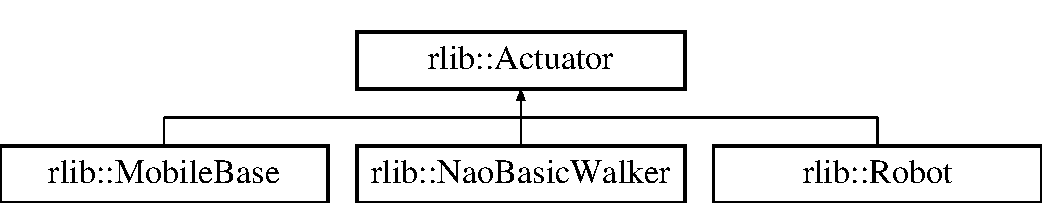
\includegraphics[height=2.000000cm]{classrlib_1_1Actuator}
\end{center}
\end{figure}
\subsection*{Public Member Functions}
\begin{DoxyCompactItemize}
\item 
\hyperlink{classrlib_1_1Actuator_a4586932cf12e921639b5186b12f87866}{Actuator} (const char $\ast$name)
\begin{DoxyCompactList}\small\item\em Constructor for the actuator class. \end{DoxyCompactList}\item 
virtual void \hyperlink{classrlib_1_1Actuator_a99eafe0706d84c5aed5d9cc3832996a5}{set\-Position} (\hyperlink{classrlib_1_1Pose}{Pose} \hyperlink{classrlib_1_1Actuator_adcce3f106abc4127382d0d9794bb7b15}{pose})=0
\begin{DoxyCompactList}\small\item\em Sets the pose of the actuator. \end{DoxyCompactList}\item 
virtual void \hyperlink{classrlib_1_1Actuator_a8495e9dee469245fa6eba719b047cb3f}{set\-Velocity} (\hyperlink{classrlib_1_1Vel}{Vel} \hyperlink{classrlib_1_1Actuator_a27372af2dd629e7b434eb541de0a13a8}{velocity})=0
\begin{DoxyCompactList}\small\item\em Sets the velocity of the actuator. \end{DoxyCompactList}\item 
void \hyperlink{classrlib_1_1Actuator_aaba68f5222df9f7878538b36daad068f}{set\-Parent} (\hyperlink{classrlib_1_1Actuator}{Actuator} $\ast$parent)
\begin{DoxyCompactList}\small\item\em Assigns the actuator parent in the kinematic chain. \end{DoxyCompactList}\item 
void \hyperlink{classrlib_1_1Actuator_a9057584b1c8855a525816f9a1a973da4}{set\-Child} (\hyperlink{classrlib_1_1Actuator}{Actuator} $\ast$child)
\begin{DoxyCompactList}\small\item\em Assigns the child actuator in the kinematic chain. \end{DoxyCompactList}\item 
void \hyperlink{classrlib_1_1Actuator_a138ade22d9534a93780f97b5c1af07a6}{set\-Frame} (\hyperlink{classrlib_1_1Transform}{Transform} tf)
\begin{DoxyCompactList}\small\item\em Sets the coordinate transformation between the parent and the sensor. \end{DoxyCompactList}\item 
void \hyperlink{classrlib_1_1Actuator_af3c3a5a5de2ab54d6b06fe223ec5e7e6}{set\-Handler} (\hyperlink{classrlib_1_1ActuatorHandler}{Actuator\-Handler} $\ast$handler)
\begin{DoxyCompactList}\small\item\em Sets the \hyperlink{classrlib_1_1ActuatorHandler}{Actuator\-Handler} for this sensor. \end{DoxyCompactList}\item 
std\-::string \hyperlink{classrlib_1_1Actuator_af4694ce3e4474e27bda1ed39cc048b6e}{get\-Name} ()
\begin{DoxyCompactList}\small\item\em Gets the actuator unique identifier. \end{DoxyCompactList}\end{DoxyCompactItemize}
\subsection*{Protected Attributes}
\begin{DoxyCompactItemize}
\item 
\hyperlink{classrlib_1_1Pose}{Pose} \hyperlink{classrlib_1_1Actuator_adcce3f106abc4127382d0d9794bb7b15}{pose}
\item 
\hyperlink{classrlib_1_1Pose}{Pose} \hyperlink{classrlib_1_1Actuator_ae0dd994c7e78e9db5580ea23d1361f4e}{pos\-Max}
\item 
\hyperlink{classrlib_1_1Pose}{Pose} \hyperlink{classrlib_1_1Actuator_a4ab8363fb4cfe849f1bb89720387d222}{pos\-Min}
\item 
\hyperlink{classrlib_1_1Vel}{Vel} \hyperlink{classrlib_1_1Actuator_a27372af2dd629e7b434eb541de0a13a8}{velocity}
\item 
\hyperlink{classrlib_1_1Vel}{Vel} \hyperlink{classrlib_1_1Actuator_a54b50a2b0f4cb61a4e5c70fa72a126dc}{vel\-Max}
\item 
\hyperlink{classrlib_1_1Vel}{Vel} \hyperlink{classrlib_1_1Actuator_ad8d95d72f27494890e16ed4ab6045f20}{vel\-Min}
\end{DoxyCompactItemize}


\subsection{Detailed Description}
Abstract class for implementing actuators. 

\hyperlink{classrlib_1_1Actuator}{Actuator} objects are used to command actuators to poses. 

\subsection{Constructor \& Destructor Documentation}
\hypertarget{classrlib_1_1Actuator_a4586932cf12e921639b5186b12f87866}{\index{rlib\-::\-Actuator@{rlib\-::\-Actuator}!Actuator@{Actuator}}
\index{Actuator@{Actuator}!rlib::Actuator@{rlib\-::\-Actuator}}
\subsubsection[{Actuator}]{\setlength{\rightskip}{0pt plus 5cm}rlib\-::\-Actuator\-::\-Actuator (
\begin{DoxyParamCaption}
\item[{const char $\ast$}]{name}
\end{DoxyParamCaption}
)}}\label{classrlib_1_1Actuator_a4586932cf12e921639b5186b12f87866}


Constructor for the actuator class. 


\begin{DoxyParams}[1]{Parameters}
\mbox{\tt in}  & {\em name} & The name for the actuator, used as a unique identifier. \\
\hline
\end{DoxyParams}


\subsection{Member Function Documentation}
\hypertarget{classrlib_1_1Actuator_af4694ce3e4474e27bda1ed39cc048b6e}{\index{rlib\-::\-Actuator@{rlib\-::\-Actuator}!get\-Name@{get\-Name}}
\index{get\-Name@{get\-Name}!rlib::Actuator@{rlib\-::\-Actuator}}
\subsubsection[{get\-Name}]{\setlength{\rightskip}{0pt plus 5cm}std\-::string rlib\-::\-Actuator\-::get\-Name (
\begin{DoxyParamCaption}
{}
\end{DoxyParamCaption}
)}}\label{classrlib_1_1Actuator_af4694ce3e4474e27bda1ed39cc048b6e}


Gets the actuator unique identifier. 

\begin{DoxyReturn}{Returns}
The name of the actuator. 
\end{DoxyReturn}
\hypertarget{classrlib_1_1Actuator_a9057584b1c8855a525816f9a1a973da4}{\index{rlib\-::\-Actuator@{rlib\-::\-Actuator}!set\-Child@{set\-Child}}
\index{set\-Child@{set\-Child}!rlib::Actuator@{rlib\-::\-Actuator}}
\subsubsection[{set\-Child}]{\setlength{\rightskip}{0pt plus 5cm}void rlib\-::\-Actuator\-::set\-Child (
\begin{DoxyParamCaption}
\item[{{\bf Actuator} $\ast$}]{child}
\end{DoxyParamCaption}
)}}\label{classrlib_1_1Actuator_a9057584b1c8855a525816f9a1a973da4}


Assigns the child actuator in the kinematic chain. 


\begin{DoxyParams}[1]{Parameters}
\mbox{\tt in}  & {\em child} & Pointer to the child actuator. \\
\hline
\end{DoxyParams}
\hypertarget{classrlib_1_1Actuator_a138ade22d9534a93780f97b5c1af07a6}{\index{rlib\-::\-Actuator@{rlib\-::\-Actuator}!set\-Frame@{set\-Frame}}
\index{set\-Frame@{set\-Frame}!rlib::Actuator@{rlib\-::\-Actuator}}
\subsubsection[{set\-Frame}]{\setlength{\rightskip}{0pt plus 5cm}void rlib\-::\-Actuator\-::set\-Frame (
\begin{DoxyParamCaption}
\item[{{\bf Transform}}]{tf}
\end{DoxyParamCaption}
)}}\label{classrlib_1_1Actuator_a138ade22d9534a93780f97b5c1af07a6}


Sets the coordinate transformation between the parent and the sensor. 


\begin{DoxyParams}[1]{Parameters}
\mbox{\tt in}  & {\em tf} & The tranformation that brings the parent frame to the sensor frame. \\
\hline
\end{DoxyParams}
\hypertarget{classrlib_1_1Actuator_af3c3a5a5de2ab54d6b06fe223ec5e7e6}{\index{rlib\-::\-Actuator@{rlib\-::\-Actuator}!set\-Handler@{set\-Handler}}
\index{set\-Handler@{set\-Handler}!rlib::Actuator@{rlib\-::\-Actuator}}
\subsubsection[{set\-Handler}]{\setlength{\rightskip}{0pt plus 5cm}void rlib\-::\-Actuator\-::set\-Handler (
\begin{DoxyParamCaption}
\item[{{\bf Actuator\-Handler} $\ast$}]{handler}
\end{DoxyParamCaption}
)}}\label{classrlib_1_1Actuator_af3c3a5a5de2ab54d6b06fe223ec5e7e6}


Sets the \hyperlink{classrlib_1_1ActuatorHandler}{Actuator\-Handler} for this sensor. 


\begin{DoxyParams}[1]{Parameters}
\mbox{\tt in}  & {\em handler} & The \hyperlink{classrlib_1_1ActuatorHandler}{Actuator\-Handler} object that interacts with the physical actuator. \\
\hline
\end{DoxyParams}
\hypertarget{classrlib_1_1Actuator_aaba68f5222df9f7878538b36daad068f}{\index{rlib\-::\-Actuator@{rlib\-::\-Actuator}!set\-Parent@{set\-Parent}}
\index{set\-Parent@{set\-Parent}!rlib::Actuator@{rlib\-::\-Actuator}}
\subsubsection[{set\-Parent}]{\setlength{\rightskip}{0pt plus 5cm}void rlib\-::\-Actuator\-::set\-Parent (
\begin{DoxyParamCaption}
\item[{{\bf Actuator} $\ast$}]{parent}
\end{DoxyParamCaption}
)}}\label{classrlib_1_1Actuator_aaba68f5222df9f7878538b36daad068f}


Assigns the actuator parent in the kinematic chain. 


\begin{DoxyParams}[1]{Parameters}
\mbox{\tt in}  & {\em parent} & Pointer to the parent actuator. \\
\hline
\end{DoxyParams}
\hypertarget{classrlib_1_1Actuator_a99eafe0706d84c5aed5d9cc3832996a5}{\index{rlib\-::\-Actuator@{rlib\-::\-Actuator}!set\-Position@{set\-Position}}
\index{set\-Position@{set\-Position}!rlib::Actuator@{rlib\-::\-Actuator}}
\subsubsection[{set\-Position}]{\setlength{\rightskip}{0pt plus 5cm}virtual void rlib\-::\-Actuator\-::set\-Position (
\begin{DoxyParamCaption}
\item[{{\bf Pose}}]{pose}
\end{DoxyParamCaption}
)\hspace{0.3cm}{\ttfamily [pure virtual]}}}\label{classrlib_1_1Actuator_a99eafe0706d84c5aed5d9cc3832996a5}


Sets the pose of the actuator. 


\begin{DoxyParams}[1]{Parameters}
\mbox{\tt in}  & {\em pose} & The pose of the actuator with respect to its origin. If the pose command contains elements outside the pose limits of the actuator then the actuator will only be commanded to setpoints within those limits. \\
\hline
\end{DoxyParams}


Implemented in \hyperlink{classrlib_1_1MobileBase_ab384dfccdcadfdfdcb4682b7361502f0}{rlib\-::\-Mobile\-Base}, and \hyperlink{classrlib_1_1NaoBasicWalker_a282dc6e13898cb72b01fbf5b133efeed}{rlib\-::\-Nao\-Basic\-Walker}.

\hypertarget{classrlib_1_1Actuator_a8495e9dee469245fa6eba719b047cb3f}{\index{rlib\-::\-Actuator@{rlib\-::\-Actuator}!set\-Velocity@{set\-Velocity}}
\index{set\-Velocity@{set\-Velocity}!rlib::Actuator@{rlib\-::\-Actuator}}
\subsubsection[{set\-Velocity}]{\setlength{\rightskip}{0pt plus 5cm}virtual void rlib\-::\-Actuator\-::set\-Velocity (
\begin{DoxyParamCaption}
\item[{{\bf Vel}}]{velocity}
\end{DoxyParamCaption}
)\hspace{0.3cm}{\ttfamily [pure virtual]}}}\label{classrlib_1_1Actuator_a8495e9dee469245fa6eba719b047cb3f}


Sets the velocity of the actuator. 


\begin{DoxyParams}[1]{Parameters}
\mbox{\tt in}  & {\em pose} & The velocity of the actuator in the local frame. \\
\hline
\end{DoxyParams}


Implemented in \hyperlink{classrlib_1_1MobileBase_a0d299cb807df63bd9cf9b259d4ce84fe}{rlib\-::\-Mobile\-Base}, and \hyperlink{classrlib_1_1NaoBasicWalker_adb9b1a9c71e0558ba57384f6b8385e1a}{rlib\-::\-Nao\-Basic\-Walker}.



\subsection{Member Data Documentation}
\hypertarget{classrlib_1_1Actuator_adcce3f106abc4127382d0d9794bb7b15}{\index{rlib\-::\-Actuator@{rlib\-::\-Actuator}!pose@{pose}}
\index{pose@{pose}!rlib::Actuator@{rlib\-::\-Actuator}}
\subsubsection[{pose}]{\setlength{\rightskip}{0pt plus 5cm}{\bf Pose} rlib\-::\-Actuator\-::pose\hspace{0.3cm}{\ttfamily [protected]}}}\label{classrlib_1_1Actuator_adcce3f106abc4127382d0d9794bb7b15}
6\-D description of actuator position with respect to the actuator origin. \hypertarget{classrlib_1_1Actuator_ae0dd994c7e78e9db5580ea23d1361f4e}{\index{rlib\-::\-Actuator@{rlib\-::\-Actuator}!pos\-Max@{pos\-Max}}
\index{pos\-Max@{pos\-Max}!rlib::Actuator@{rlib\-::\-Actuator}}
\subsubsection[{pos\-Max}]{\setlength{\rightskip}{0pt plus 5cm}{\bf Pose} rlib\-::\-Actuator\-::pos\-Max\hspace{0.3cm}{\ttfamily [protected]}}}\label{classrlib_1_1Actuator_ae0dd994c7e78e9db5580ea23d1361f4e}
\hyperlink{classrlib_1_1Pose}{Pose} maximum limits for the actuator. \hypertarget{classrlib_1_1Actuator_a4ab8363fb4cfe849f1bb89720387d222}{\index{rlib\-::\-Actuator@{rlib\-::\-Actuator}!pos\-Min@{pos\-Min}}
\index{pos\-Min@{pos\-Min}!rlib::Actuator@{rlib\-::\-Actuator}}
\subsubsection[{pos\-Min}]{\setlength{\rightskip}{0pt plus 5cm}{\bf Pose} rlib\-::\-Actuator\-::pos\-Min\hspace{0.3cm}{\ttfamily [protected]}}}\label{classrlib_1_1Actuator_a4ab8363fb4cfe849f1bb89720387d222}
\hyperlink{classrlib_1_1Pose}{Pose} minimum limits for the actuator. \hypertarget{classrlib_1_1Actuator_a54b50a2b0f4cb61a4e5c70fa72a126dc}{\index{rlib\-::\-Actuator@{rlib\-::\-Actuator}!vel\-Max@{vel\-Max}}
\index{vel\-Max@{vel\-Max}!rlib::Actuator@{rlib\-::\-Actuator}}
\subsubsection[{vel\-Max}]{\setlength{\rightskip}{0pt plus 5cm}{\bf Vel} rlib\-::\-Actuator\-::vel\-Max\hspace{0.3cm}{\ttfamily [protected]}}}\label{classrlib_1_1Actuator_a54b50a2b0f4cb61a4e5c70fa72a126dc}
Velocity maximum limits for the actuator. \hypertarget{classrlib_1_1Actuator_ad8d95d72f27494890e16ed4ab6045f20}{\index{rlib\-::\-Actuator@{rlib\-::\-Actuator}!vel\-Min@{vel\-Min}}
\index{vel\-Min@{vel\-Min}!rlib::Actuator@{rlib\-::\-Actuator}}
\subsubsection[{vel\-Min}]{\setlength{\rightskip}{0pt plus 5cm}{\bf Vel} rlib\-::\-Actuator\-::vel\-Min\hspace{0.3cm}{\ttfamily [protected]}}}\label{classrlib_1_1Actuator_ad8d95d72f27494890e16ed4ab6045f20}
Velocity minimum limits for the actuator. \hypertarget{classrlib_1_1Actuator_a27372af2dd629e7b434eb541de0a13a8}{\index{rlib\-::\-Actuator@{rlib\-::\-Actuator}!velocity@{velocity}}
\index{velocity@{velocity}!rlib::Actuator@{rlib\-::\-Actuator}}
\subsubsection[{velocity}]{\setlength{\rightskip}{0pt plus 5cm}{\bf Vel} rlib\-::\-Actuator\-::velocity\hspace{0.3cm}{\ttfamily [protected]}}}\label{classrlib_1_1Actuator_a27372af2dd629e7b434eb541de0a13a8}
6\-D description of actuator velocity with respect to the actuator origin. 

The documentation for this class was generated from the following files\-:\begin{DoxyCompactItemize}
\item 
include/rlib\-\_\-actuator.\-hpp\item 
src/rlib\-\_\-actuator.\-cpp\end{DoxyCompactItemize}

\hypertarget{unionhokuyo_1_1fpn4b__t}{\section{hokuyo\-:\-:fpn4b\-\_\-t Union Reference}
\label{unionhokuyo_1_1fpn4b__t}\index{hokuyo\-::fpn4b\-\_\-t@{hokuyo\-::fpn4b\-\_\-t}}
}
\subsection*{Public Attributes}
\begin{DoxyCompactItemize}
\item 
\hypertarget{unionhokuyo_1_1fpn4b__t_a22afb0bd4af1b752e365f67335f49e97}{uint8\-\_\-t {\bfseries bytes} \mbox{[}8\-U\-L\mbox{]}}\label{unionhokuyo_1_1fpn4b__t_a22afb0bd4af1b752e365f67335f49e97}

\item 
\hypertarget{unionhokuyo_1_1fpn4b__t_a14c818fca2156565697f67945b96acca}{double {\bfseries fpn}}\label{unionhokuyo_1_1fpn4b__t_a14c818fca2156565697f67945b96acca}

\end{DoxyCompactItemize}


The documentation for this union was generated from the following file\-:\begin{DoxyCompactItemize}
\item 
src/hokuyo\-\_\-client.\-cpp\end{DoxyCompactItemize}

\hypertarget{classrlib_1_1HokuyoLidarHandlerIP}{\section{rlib\-:\-:Hokuyo\-Lidar\-Handler\-I\-P Class Reference}
\label{classrlib_1_1HokuyoLidarHandlerIP}\index{rlib\-::\-Hokuyo\-Lidar\-Handler\-I\-P@{rlib\-::\-Hokuyo\-Lidar\-Handler\-I\-P}}
}


Hokuyo Lidar Handler class using I\-P connected Lidar.  




{\ttfamily \#include $<$rlib\-\_\-sensor.\-hpp$>$}

Inheritance diagram for rlib\-:\-:Hokuyo\-Lidar\-Handler\-I\-P\-:\begin{figure}[H]
\begin{center}
\leavevmode
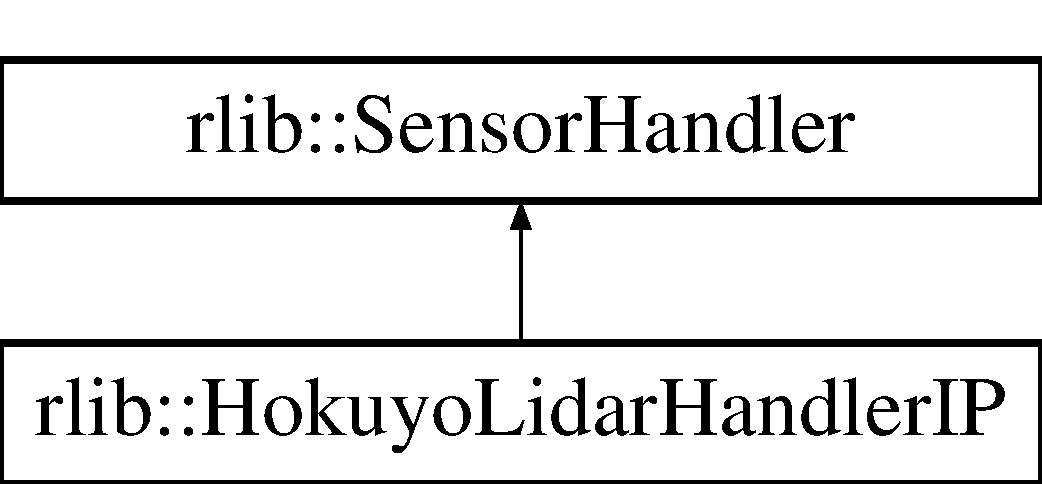
\includegraphics[height=2.000000cm]{classrlib_1_1HokuyoLidarHandlerIP}
\end{center}
\end{figure}
\subsection*{Public Member Functions}
\begin{DoxyCompactItemize}
\item 
\hyperlink{classrlib_1_1HokuyoLidarHandlerIP_a5670fe812188c2a47f2095161ed6d5a5}{Hokuyo\-Lidar\-Handler\-I\-P} (const char $\ast$ip, const char $\ast$port)
\begin{DoxyCompactList}\small\item\em Constructor for I\-P version of Hokoyu Lidar Handler. \end{DoxyCompactList}\item 
\hypertarget{classrlib_1_1HokuyoLidarHandlerIP_a379dbeec9ace02bb0d4840509f009576}{void \hyperlink{classrlib_1_1HokuyoLidarHandlerIP_a379dbeec9ace02bb0d4840509f009576}{start\-Sensor} ()}\label{classrlib_1_1HokuyoLidarHandlerIP_a379dbeec9ace02bb0d4840509f009576}

\begin{DoxyCompactList}\small\item\em Initiates communication with the Lidar. \end{DoxyCompactList}\item 
\hypertarget{classrlib_1_1HokuyoLidarHandlerIP_aafe7200d26d5a38642da2d58e6ccf2b3}{void \hyperlink{classrlib_1_1HokuyoLidarHandlerIP_aafe7200d26d5a38642da2d58e6ccf2b3}{stop\-Sensor} ()}\label{classrlib_1_1HokuyoLidarHandlerIP_aafe7200d26d5a38642da2d58e6ccf2b3}

\begin{DoxyCompactList}\small\item\em Terminates Lidar connection. \end{DoxyCompactList}\item 
\hyperlink{classrlib_1_1SensorData}{Sensor\-Data} $\ast$ \hyperlink{classrlib_1_1HokuyoLidarHandlerIP_af1b24513e31b16fb97b9a9124f29bc40}{get\-Data} ()
\begin{DoxyCompactList}\small\item\em Gets range and angle data from the sensor. \end{DoxyCompactList}\end{DoxyCompactItemize}


\subsection{Detailed Description}
Hokuyo Lidar Handler class using I\-P connected Lidar. 

This is a handler class derived from the \hyperlink{classrlib_1_1SensorHandler}{rlib\-::\-Sensor\-Handler} class. It is designed for use with the Hokuyo Lidar U\-R\-G-\/04\-L\-X-\/\-U\-G01. The Lidar is started using the Python lidar\-\_\-server\-\_\-tester.\-py written by Abhimanyu Ghosh. This client handler is a wrapper class for the client library hokuyo\-\_\-client.\-cpp written by Brian Cairl. 

\subsection{Constructor \& Destructor Documentation}
\hypertarget{classrlib_1_1HokuyoLidarHandlerIP_a5670fe812188c2a47f2095161ed6d5a5}{\index{rlib\-::\-Hokuyo\-Lidar\-Handler\-I\-P@{rlib\-::\-Hokuyo\-Lidar\-Handler\-I\-P}!Hokuyo\-Lidar\-Handler\-I\-P@{Hokuyo\-Lidar\-Handler\-I\-P}}
\index{Hokuyo\-Lidar\-Handler\-I\-P@{Hokuyo\-Lidar\-Handler\-I\-P}!rlib::HokuyoLidarHandlerIP@{rlib\-::\-Hokuyo\-Lidar\-Handler\-I\-P}}
\subsubsection[{Hokuyo\-Lidar\-Handler\-I\-P}]{\setlength{\rightskip}{0pt plus 5cm}rlib\-::\-Hokuyo\-Lidar\-Handler\-I\-P\-::\-Hokuyo\-Lidar\-Handler\-I\-P (
\begin{DoxyParamCaption}
\item[{const char $\ast$}]{ip, }
\item[{const char $\ast$}]{port}
\end{DoxyParamCaption}
)}}\label{classrlib_1_1HokuyoLidarHandlerIP_a5670fe812188c2a47f2095161ed6d5a5}


Constructor for I\-P version of Hokoyu Lidar Handler. 

$\ast$$\ast$$\ast$ \hyperlink{classrlib_1_1HokuyoLidarHandlerIP}{Hokuyo\-Lidar\-Handler\-I\-P} Class $\ast$$\ast$$\ast$///

The constructor for the handler needs the I\-P address and port number that the Lidar is running on. 
\begin{DoxyParams}[1]{Parameters}
\mbox{\tt in}  & {\em ip} & This is the I\-P address of the computer that the Lidar is connected to. \\
\hline
\mbox{\tt in}  & {\em port} & This is the port number of the Lidar on the computer. \\
\hline
\end{DoxyParams}


\subsection{Member Function Documentation}
\hypertarget{classrlib_1_1HokuyoLidarHandlerIP_af1b24513e31b16fb97b9a9124f29bc40}{\index{rlib\-::\-Hokuyo\-Lidar\-Handler\-I\-P@{rlib\-::\-Hokuyo\-Lidar\-Handler\-I\-P}!get\-Data@{get\-Data}}
\index{get\-Data@{get\-Data}!rlib::HokuyoLidarHandlerIP@{rlib\-::\-Hokuyo\-Lidar\-Handler\-I\-P}}
\subsubsection[{get\-Data}]{\setlength{\rightskip}{0pt plus 5cm}{\bf Sensor\-Data} $\ast$ rlib\-::\-Hokuyo\-Lidar\-Handler\-I\-P\-::get\-Data (
\begin{DoxyParamCaption}
{}
\end{DoxyParamCaption}
)\hspace{0.3cm}{\ttfamily [virtual]}}}\label{classrlib_1_1HokuyoLidarHandlerIP_af1b24513e31b16fb97b9a9124f29bc40}


Gets range and angle data from the sensor. 

Requests new sensor data from the Lidar. This is a blocking function. \begin{DoxyReturn}{Returns}
The range and angle data packed into the \hyperlink{classrlib_1_1SensorData}{rlib\-::\-Sensor\-Data} format. 
\end{DoxyReturn}


Implements \hyperlink{classrlib_1_1SensorHandler_a7f9c3e855f436aab794969b3b5cc3193}{rlib\-::\-Sensor\-Handler}.



The documentation for this class was generated from the following files\-:\begin{DoxyCompactItemize}
\item 
include/rlib\-\_\-sensor.\-hpp\item 
src/rlib\-\_\-sensor.\-cpp\end{DoxyCompactItemize}

\hypertarget{classrlib_1_1ImageData}{\section{rlib\-:\-:Image\-Data Class Reference}
\label{classrlib_1_1ImageData}\index{rlib\-::\-Image\-Data@{rlib\-::\-Image\-Data}}
}
Inheritance diagram for rlib\-:\-:Image\-Data\-:\begin{figure}[H]
\begin{center}
\leavevmode
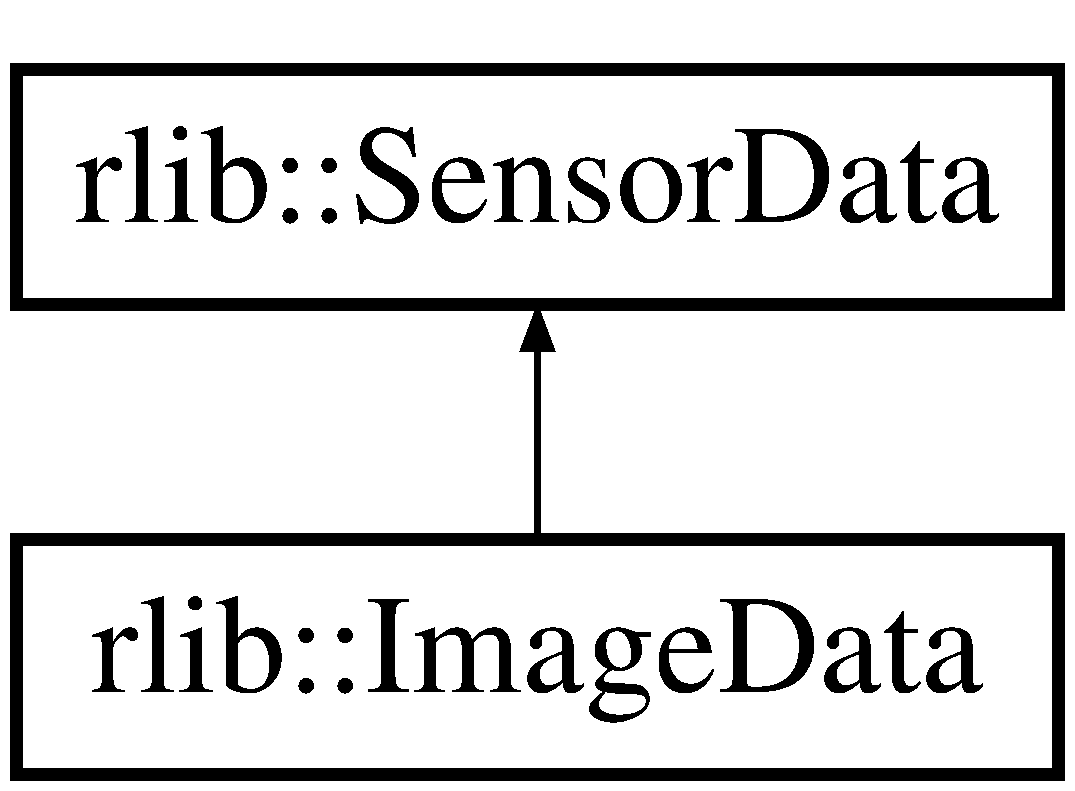
\includegraphics[height=2.000000cm]{classrlib_1_1ImageData}
\end{center}
\end{figure}


The documentation for this class was generated from the following file\-:\begin{DoxyCompactItemize}
\item 
include/rlib\-\_\-sensor.\-hpp\end{DoxyCompactItemize}

\hypertarget{classrlib_1_1InfraredData}{\section{rlib\-:\-:Infrared\-Data Class Reference}
\label{classrlib_1_1InfraredData}\index{rlib\-::\-Infrared\-Data@{rlib\-::\-Infrared\-Data}}
}
Inheritance diagram for rlib\-:\-:Infrared\-Data\-:\begin{figure}[H]
\begin{center}
\leavevmode
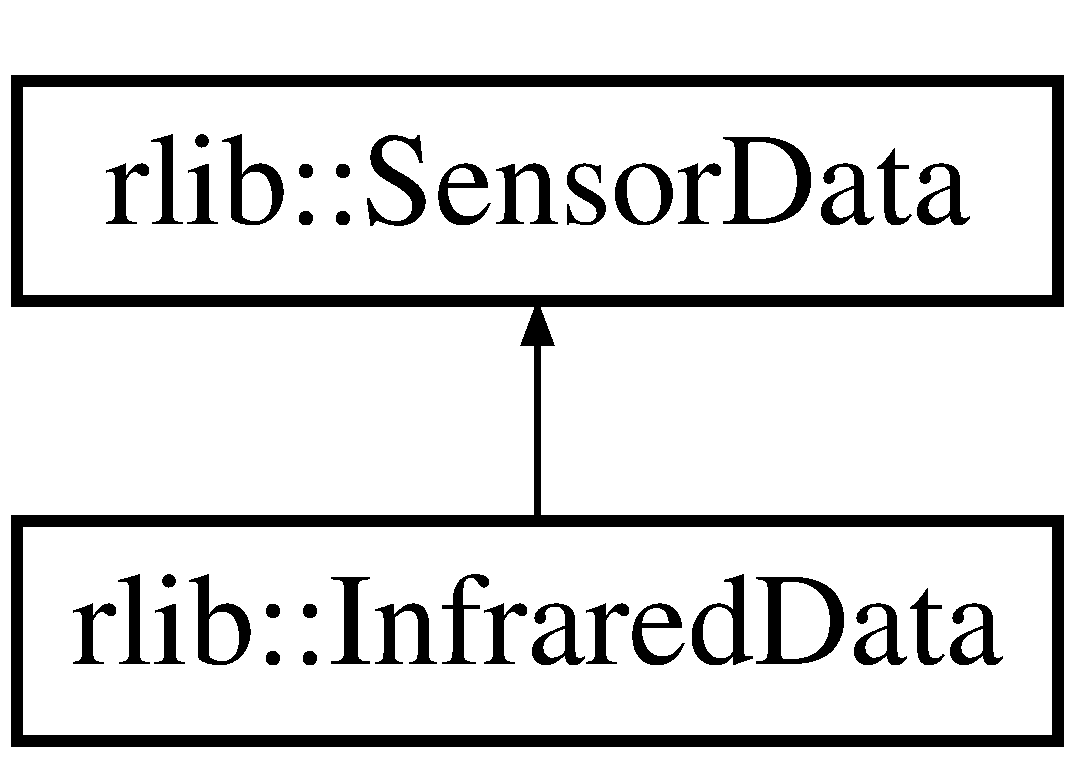
\includegraphics[height=2.000000cm]{classrlib_1_1InfraredData}
\end{center}
\end{figure}


The documentation for this class was generated from the following file\-:\begin{DoxyCompactItemize}
\item 
include/rlib\-\_\-sensor.\-hpp\end{DoxyCompactItemize}

\hypertarget{classrlib_1_1Lidar}{\section{rlib\-:\-:Lidar Class Reference}
\label{classrlib_1_1Lidar}\index{rlib\-::\-Lidar@{rlib\-::\-Lidar}}
}


$\ast$$\ast$$\ast$ Some Basic \hyperlink{classrlib_1_1Sensor}{Sensor} Derivative Classes $\ast$$\ast$$\ast$///  




{\ttfamily \#include $<$rlib\-\_\-sensor.\-hpp$>$}

Inheritance diagram for rlib\-:\-:Lidar\-:\begin{figure}[H]
\begin{center}
\leavevmode
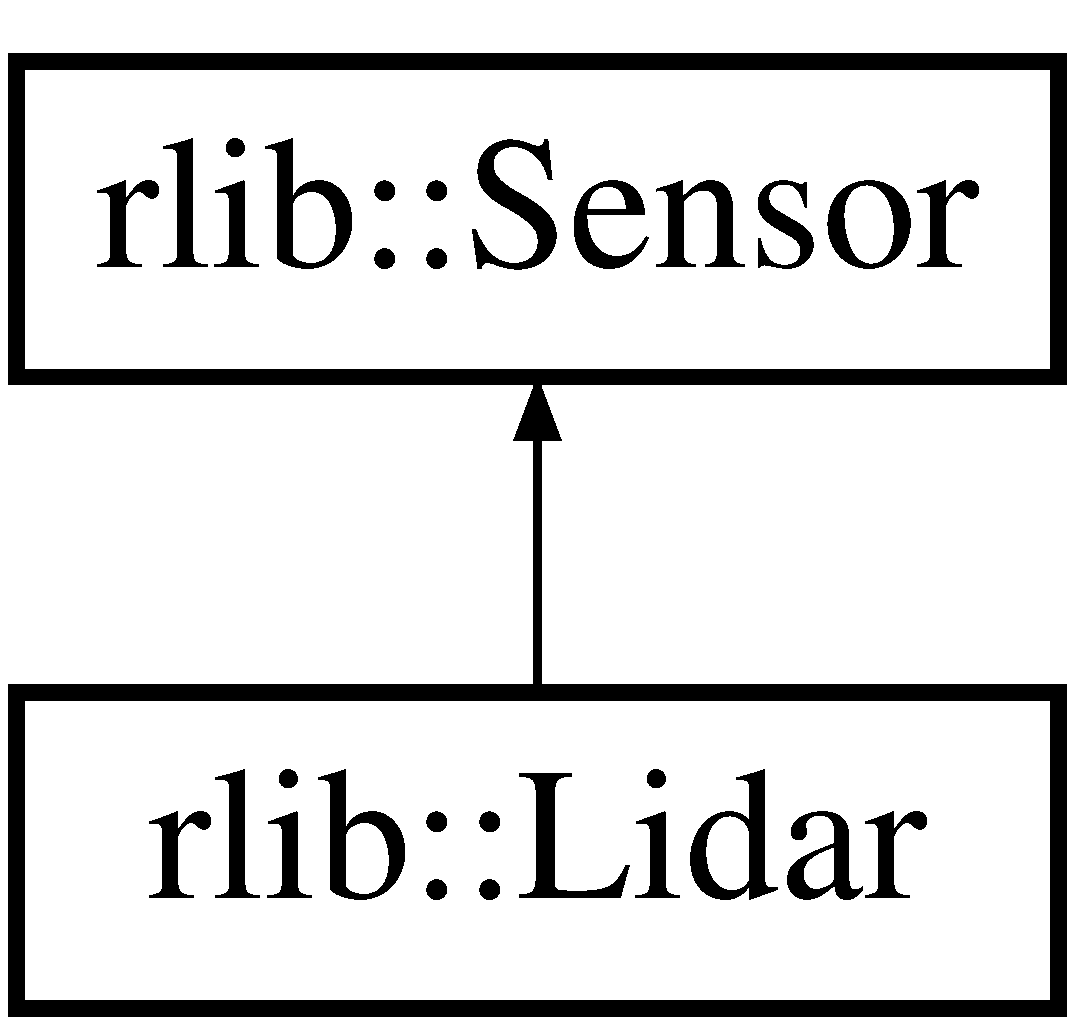
\includegraphics[height=2.000000cm]{classrlib_1_1Lidar}
\end{center}
\end{figure}
\subsection*{Public Member Functions}
\begin{DoxyCompactItemize}
\item 
\hypertarget{classrlib_1_1Lidar_abcf72f8479bf7869780a407d7f5eb636}{\hyperlink{classrlib_1_1Lidar_abcf72f8479bf7869780a407d7f5eb636}{Lidar} (const char $\ast$name)}\label{classrlib_1_1Lidar_abcf72f8479bf7869780a407d7f5eb636}

\begin{DoxyCompactList}\small\item\em $\ast$$\ast$$\ast$ \hyperlink{classrlib_1_1Lidar}{Lidar} Class $\ast$$\ast$$\ast$/// \end{DoxyCompactList}\item 
\hypertarget{classrlib_1_1Lidar_a61f34281376ee91d1f85ac6daae357b1}{void {\bfseries set\-Frame} (\hyperlink{classrlib_1_1Transform}{Transform} tf)}\label{classrlib_1_1Lidar_a61f34281376ee91d1f85ac6daae357b1}

\item 
\hypertarget{classrlib_1_1Lidar_adca8ff96e94bbb7490063c16ebf1c2e9}{void {\bfseries start\-Sensor} ()}\label{classrlib_1_1Lidar_adca8ff96e94bbb7490063c16ebf1c2e9}

\item 
\hypertarget{classrlib_1_1Lidar_aff59b61b1d295b8ac5fa6d7f5d3081c5}{void {\bfseries stop\-Sensor} ()}\label{classrlib_1_1Lidar_aff59b61b1d295b8ac5fa6d7f5d3081c5}

\item 
\hypertarget{classrlib_1_1Lidar_af1622c97196bab2330e9e4cfe42d1c51}{\hyperlink{classrlib_1_1SensorData}{Sensor\-Data} {\bfseries get\-Data} ()}\label{classrlib_1_1Lidar_af1622c97196bab2330e9e4cfe42d1c51}

\end{DoxyCompactItemize}


\subsection{Detailed Description}
$\ast$$\ast$$\ast$ Some Basic \hyperlink{classrlib_1_1Sensor}{Sensor} Derivative Classes $\ast$$\ast$$\ast$/// 

The documentation for this class was generated from the following files\-:\begin{DoxyCompactItemize}
\item 
include/rlib\-\_\-sensor.\-hpp\item 
src/rlib\-\_\-sensor.\-cpp\end{DoxyCompactItemize}

\hypertarget{classrlib_1_1LidarData}{\section{rlib\-:\-:Lidar\-Data Class Reference}
\label{classrlib_1_1LidarData}\index{rlib\-::\-Lidar\-Data@{rlib\-::\-Lidar\-Data}}
}


\hyperlink{classrlib_1_1LidarData}{Lidar\-Data} class for getting data from a Lidar \hyperlink{classrlib_1_1Sensor}{Sensor}.  




{\ttfamily \#include $<$rlib\-\_\-sensor.\-hpp$>$}

Inheritance diagram for rlib\-:\-:Lidar\-Data\-:\begin{figure}[H]
\begin{center}
\leavevmode
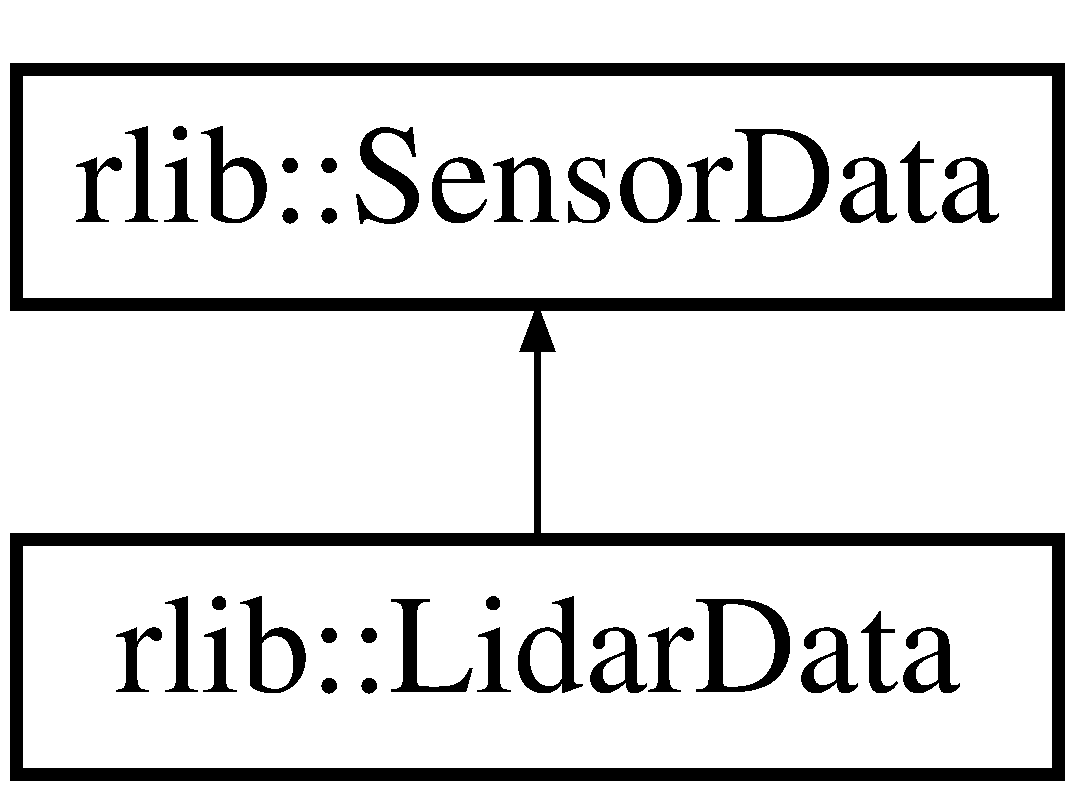
\includegraphics[height=2.000000cm]{classrlib_1_1LidarData}
\end{center}
\end{figure}
\subsection*{Public Member Functions}
\begin{DoxyCompactItemize}
\item 
\hyperlink{classrlib_1_1LidarData_a57b4749e1274030136fce1e5fbbca33d}{Lidar\-Data} (std\-::vector$<$ float $>$ \&ranges, std\-::vector$<$ float $>$ \&angles)
\begin{DoxyCompactList}\small\item\em Constructor for \hyperlink{classrlib_1_1LidarData}{Lidar\-Data} objects. \end{DoxyCompactList}\item 
size\-\_\-t \hyperlink{classrlib_1_1LidarData_abf37f41dee75528211a93833e2d68520}{size} ()
\begin{DoxyCompactList}\small\item\em Returns number of data elements. \end{DoxyCompactList}\item 
float \hyperlink{classrlib_1_1LidarData_a7c0a03b228b5b85e81b35f2cc61e6008}{get\-Range} (float angle)
\begin{DoxyCompactList}\small\item\em Get a range for a given angle. If no angle is found, method will return range to the closest angle. \end{DoxyCompactList}\item 
const Eigen\-::\-Matrix$<$ float, \\*
2, Eigen\-::\-Dynamic $>$ \& \hyperlink{classrlib_1_1LidarData_a4249c865a00c72fe80c8a210667c2ca4}{get\-Data} ()
\begin{DoxyCompactList}\small\item\em Get the sensor data. \end{DoxyCompactList}\item 
void \hyperlink{classrlib_1_1LidarData_a1d9dc0bbc59f528f3d76492fd5aec816}{print\-To\-Stream} (std\-::ostream \&os)
\begin{DoxyCompactList}\small\item\em Print function for streams. \end{DoxyCompactList}\end{DoxyCompactItemize}
\subsection*{Friends}
\begin{DoxyCompactItemize}
\item 
\hypertarget{classrlib_1_1LidarData_ac142a9d8c3161d74c8d3d39c093ecde4}{std\-::ostream \& \hyperlink{classrlib_1_1LidarData_ac142a9d8c3161d74c8d3d39c093ecde4}{operator$<$$<$} (std\-::ostream \&os, \hyperlink{classrlib_1_1LidarData}{Lidar\-Data} \&data)}\label{classrlib_1_1LidarData_ac142a9d8c3161d74c8d3d39c093ecde4}

\begin{DoxyCompactList}\small\item\em Print operator for Lidar Data. \end{DoxyCompactList}\end{DoxyCompactItemize}


\subsection{Detailed Description}
\hyperlink{classrlib_1_1LidarData}{Lidar\-Data} class for getting data from a Lidar \hyperlink{classrlib_1_1Sensor}{Sensor}. 

This class is for encapsulating the data produced by a Lidar \hyperlink{classrlib_1_1Sensor}{Sensor} and making it easy to access the data in different ways. 

\subsection{Constructor \& Destructor Documentation}
\hypertarget{classrlib_1_1LidarData_a57b4749e1274030136fce1e5fbbca33d}{\index{rlib\-::\-Lidar\-Data@{rlib\-::\-Lidar\-Data}!Lidar\-Data@{Lidar\-Data}}
\index{Lidar\-Data@{Lidar\-Data}!rlib::LidarData@{rlib\-::\-Lidar\-Data}}
\subsubsection[{Lidar\-Data}]{\setlength{\rightskip}{0pt plus 5cm}rlib\-::\-Lidar\-Data\-::\-Lidar\-Data (
\begin{DoxyParamCaption}
\item[{std\-::vector$<$ float $>$ \&}]{ranges, }
\item[{std\-::vector$<$ float $>$ \&}]{angles}
\end{DoxyParamCaption}
)}}\label{classrlib_1_1LidarData_a57b4749e1274030136fce1e5fbbca33d}


Constructor for \hyperlink{classrlib_1_1LidarData}{Lidar\-Data} objects. 

$\ast$$\ast$$\ast$ Lidar Data Class $\ast$$\ast$$\ast$///

The constructor for the needs a std\-::vector of ranges and angles. Each vector must be the same length and the indices must correspond with each others data. The vectors do not need to be sorted by angle, and in general are not. 
\begin{DoxyParams}[1]{Parameters}
\mbox{\tt in}  & {\em ranges} & This is the I\-P address of the computer that the Lidar is connected to. \\
\hline
\mbox{\tt in}  & {\em angles} & This is the port number of the Lidar on the computer. \\
\hline
\end{DoxyParams}


\subsection{Member Function Documentation}
\hypertarget{classrlib_1_1LidarData_a4249c865a00c72fe80c8a210667c2ca4}{\index{rlib\-::\-Lidar\-Data@{rlib\-::\-Lidar\-Data}!get\-Data@{get\-Data}}
\index{get\-Data@{get\-Data}!rlib::LidarData@{rlib\-::\-Lidar\-Data}}
\subsubsection[{get\-Data}]{\setlength{\rightskip}{0pt plus 5cm}const Eigen\-::\-Matrix$<$ float, 2, Eigen\-::\-Dynamic $>$ \& rlib\-::\-Lidar\-Data\-::get\-Data (
\begin{DoxyParamCaption}
{}
\end{DoxyParamCaption}
)}}\label{classrlib_1_1LidarData_a4249c865a00c72fe80c8a210667c2ca4}


Get the sensor data. 

\begin{DoxyReturn}{Returns}
A 2x2 Matrix of floats of ranges and angles in meters and radians. The ranges are on the first row and their corresponding angles are on the second row. 
\end{DoxyReturn}
\hypertarget{classrlib_1_1LidarData_a7c0a03b228b5b85e81b35f2cc61e6008}{\index{rlib\-::\-Lidar\-Data@{rlib\-::\-Lidar\-Data}!get\-Range@{get\-Range}}
\index{get\-Range@{get\-Range}!rlib::LidarData@{rlib\-::\-Lidar\-Data}}
\subsubsection[{get\-Range}]{\setlength{\rightskip}{0pt plus 5cm}float rlib\-::\-Lidar\-Data\-::get\-Range (
\begin{DoxyParamCaption}
\item[{float}]{angle}
\end{DoxyParamCaption}
)}}\label{classrlib_1_1LidarData_a7c0a03b228b5b85e81b35f2cc61e6008}


Get a range for a given angle. If no angle is found, method will return range to the closest angle. 


\begin{DoxyParams}[1]{Parameters}
\mbox{\tt in}  & {\em angle} & The angle in radians to get a range for. \\
\hline
\end{DoxyParams}
\begin{DoxyReturn}{Returns}
The range in meters. 
\end{DoxyReturn}
\hypertarget{classrlib_1_1LidarData_a1d9dc0bbc59f528f3d76492fd5aec816}{\index{rlib\-::\-Lidar\-Data@{rlib\-::\-Lidar\-Data}!print\-To\-Stream@{print\-To\-Stream}}
\index{print\-To\-Stream@{print\-To\-Stream}!rlib::LidarData@{rlib\-::\-Lidar\-Data}}
\subsubsection[{print\-To\-Stream}]{\setlength{\rightskip}{0pt plus 5cm}void rlib\-::\-Lidar\-Data\-::print\-To\-Stream (
\begin{DoxyParamCaption}
\item[{std\-::ostream \&}]{os}
\end{DoxyParamCaption}
)\hspace{0.3cm}{\ttfamily [virtual]}}}\label{classrlib_1_1LidarData_a1d9dc0bbc59f528f3d76492fd5aec816}


Print function for streams. 


\begin{DoxyParams}[1]{Parameters}
\mbox{\tt in}  & {\em os} & The output stream that the data should be printed to. \\
\hline
\end{DoxyParams}


Implements \hyperlink{classrlib_1_1SensorData}{rlib\-::\-Sensor\-Data}.

\hypertarget{classrlib_1_1LidarData_abf37f41dee75528211a93833e2d68520}{\index{rlib\-::\-Lidar\-Data@{rlib\-::\-Lidar\-Data}!size@{size}}
\index{size@{size}!rlib::LidarData@{rlib\-::\-Lidar\-Data}}
\subsubsection[{size}]{\setlength{\rightskip}{0pt plus 5cm}size\-\_\-t rlib\-::\-Lidar\-Data\-::size (
\begin{DoxyParamCaption}
{}
\end{DoxyParamCaption}
)}}\label{classrlib_1_1LidarData_abf37f41dee75528211a93833e2d68520}


Returns number of data elements. 

\begin{DoxyReturn}{Returns}
The number of range angle pairs in the set. 
\end{DoxyReturn}


The documentation for this class was generated from the following files\-:\begin{DoxyCompactItemize}
\item 
include/rlib\-\_\-sensor.\-hpp\item 
src/rlib\-\_\-sensor.\-cpp\end{DoxyCompactItemize}

\hypertarget{classrlib_1_1MobileBase}{\section{rlib\-:\-:Mobile\-Base Class Reference}
\label{classrlib_1_1MobileBase}\index{rlib\-::\-Mobile\-Base@{rlib\-::\-Mobile\-Base}}
}
Inheritance diagram for rlib\-:\-:Mobile\-Base\-:\begin{figure}[H]
\begin{center}
\leavevmode
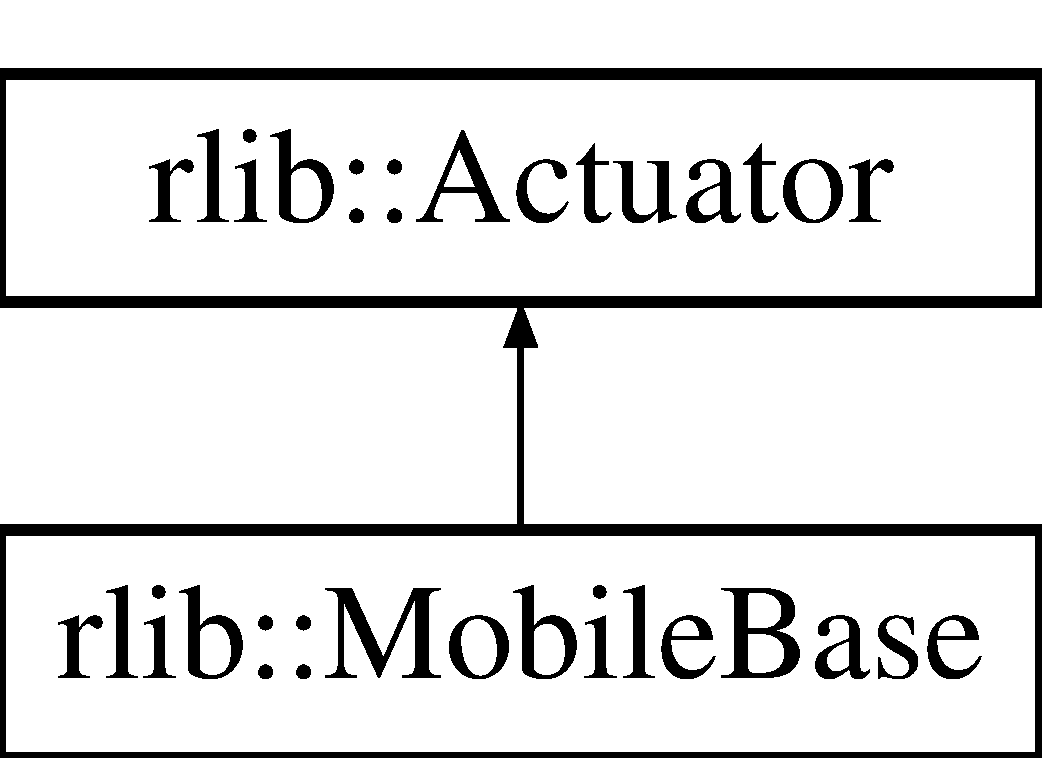
\includegraphics[height=2.000000cm]{classrlib_1_1MobileBase}
\end{center}
\end{figure}
\subsection*{Public Member Functions}
\begin{DoxyCompactItemize}
\item 
\hypertarget{classrlib_1_1MobileBase_a7bd9b6898b967ea5eee27f64a4a62063}{{\bfseries Mobile\-Base} (const char $\ast$name)}\label{classrlib_1_1MobileBase_a7bd9b6898b967ea5eee27f64a4a62063}

\item 
void \hyperlink{classrlib_1_1MobileBase_ab384dfccdcadfdfdcb4682b7361502f0}{set\-Position} (\hyperlink{classrlib_1_1Pose}{Pose} \hyperlink{classrlib_1_1Actuator_adcce3f106abc4127382d0d9794bb7b15}{pose})
\begin{DoxyCompactList}\small\item\em Sets the pose of the actuator. \end{DoxyCompactList}\item 
void \hyperlink{classrlib_1_1MobileBase_a0d299cb807df63bd9cf9b259d4ce84fe}{set\-Velocity} (\hyperlink{classrlib_1_1Vel}{Vel} \hyperlink{classrlib_1_1Actuator_a27372af2dd629e7b434eb541de0a13a8}{velocity})
\begin{DoxyCompactList}\small\item\em Sets the velocity of the actuator. \end{DoxyCompactList}\end{DoxyCompactItemize}
\subsection*{Additional Inherited Members}


\subsection{Member Function Documentation}
\hypertarget{classrlib_1_1MobileBase_ab384dfccdcadfdfdcb4682b7361502f0}{\index{rlib\-::\-Mobile\-Base@{rlib\-::\-Mobile\-Base}!set\-Position@{set\-Position}}
\index{set\-Position@{set\-Position}!rlib::MobileBase@{rlib\-::\-Mobile\-Base}}
\subsubsection[{set\-Position}]{\setlength{\rightskip}{0pt plus 5cm}void rlib\-::\-Mobile\-Base\-::set\-Position (
\begin{DoxyParamCaption}
\item[{{\bf Pose}}]{pose}
\end{DoxyParamCaption}
)\hspace{0.3cm}{\ttfamily [virtual]}}}\label{classrlib_1_1MobileBase_ab384dfccdcadfdfdcb4682b7361502f0}


Sets the pose of the actuator. 


\begin{DoxyParams}[1]{Parameters}
\mbox{\tt in}  & {\em pose} & The pose of the actuator with respect to its origin. If the pose command contains elements outside the pose limits of the actuator then the actuator will only be commanded to setpoints within those limits. \\
\hline
\end{DoxyParams}


Implements \hyperlink{classrlib_1_1Actuator_a99eafe0706d84c5aed5d9cc3832996a5}{rlib\-::\-Actuator}.

\hypertarget{classrlib_1_1MobileBase_a0d299cb807df63bd9cf9b259d4ce84fe}{\index{rlib\-::\-Mobile\-Base@{rlib\-::\-Mobile\-Base}!set\-Velocity@{set\-Velocity}}
\index{set\-Velocity@{set\-Velocity}!rlib::MobileBase@{rlib\-::\-Mobile\-Base}}
\subsubsection[{set\-Velocity}]{\setlength{\rightskip}{0pt plus 5cm}void rlib\-::\-Mobile\-Base\-::set\-Velocity (
\begin{DoxyParamCaption}
\item[{{\bf Vel}}]{velocity}
\end{DoxyParamCaption}
)\hspace{0.3cm}{\ttfamily [virtual]}}}\label{classrlib_1_1MobileBase_a0d299cb807df63bd9cf9b259d4ce84fe}


Sets the velocity of the actuator. 


\begin{DoxyParams}[1]{Parameters}
\mbox{\tt in}  & {\em pose} & The velocity of the actuator in the local frame. \\
\hline
\end{DoxyParams}


Implements \hyperlink{classrlib_1_1Actuator_a8495e9dee469245fa6eba719b047cb3f}{rlib\-::\-Actuator}.



The documentation for this class was generated from the following files\-:\begin{DoxyCompactItemize}
\item 
include/rlib\-\_\-actuator.\-hpp\item 
src/rlib\-\_\-actuator.\-cpp\end{DoxyCompactItemize}

\hypertarget{classrlib_1_1NaoBasicWalker}{\section{rlib\-:\-:Nao\-Basic\-Walker Class Reference}
\label{classrlib_1_1NaoBasicWalker}\index{rlib\-::\-Nao\-Basic\-Walker@{rlib\-::\-Nao\-Basic\-Walker}}
}
Inheritance diagram for rlib\-:\-:Nao\-Basic\-Walker\-:\begin{figure}[H]
\begin{center}
\leavevmode
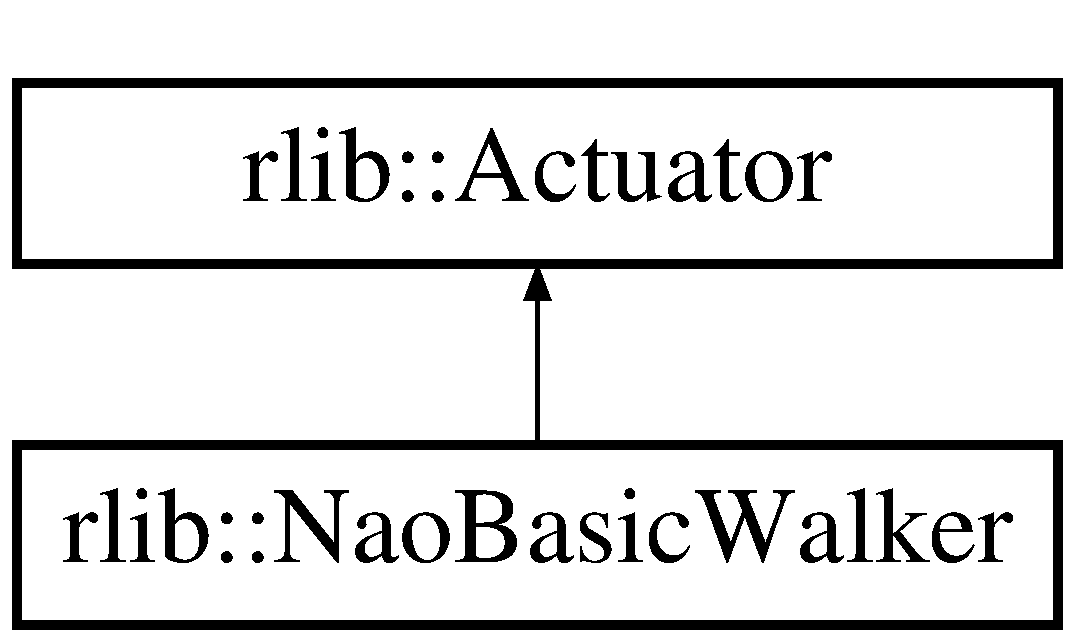
\includegraphics[height=2.000000cm]{classrlib_1_1NaoBasicWalker}
\end{center}
\end{figure}
\subsection*{Public Member Functions}
\begin{DoxyCompactItemize}
\item 
\hypertarget{classrlib_1_1NaoBasicWalker_a43bdf705d8aeb9cdd8638cee899303b3}{{\bfseries Nao\-Basic\-Walker} (const char $\ast$name)}\label{classrlib_1_1NaoBasicWalker_a43bdf705d8aeb9cdd8638cee899303b3}

\item 
\hypertarget{classrlib_1_1NaoBasicWalker_a282dc6e13898cb72b01fbf5b133efeed}{void {\bfseries set\-Position} (\hyperlink{classrlib_1_1Pose}{Pose} pose)}\label{classrlib_1_1NaoBasicWalker_a282dc6e13898cb72b01fbf5b133efeed}

\item 
\hypertarget{classrlib_1_1NaoBasicWalker_adb9b1a9c71e0558ba57384f6b8385e1a}{void {\bfseries set\-Velocity} (\hyperlink{classrlib_1_1Vel}{Vel} velocity)}\label{classrlib_1_1NaoBasicWalker_adb9b1a9c71e0558ba57384f6b8385e1a}

\end{DoxyCompactItemize}
\subsection*{Additional Inherited Members}


The documentation for this class was generated from the following files\-:\begin{DoxyCompactItemize}
\item 
include/rlib\-\_\-nao.\-hpp\item 
src/rlib\-\_\-nao.\-cpp\end{DoxyCompactItemize}

\hypertarget{classrlib_1_1PointCloudData}{\section{rlib\-:\-:Point\-Cloud\-Data Class Reference}
\label{classrlib_1_1PointCloudData}\index{rlib\-::\-Point\-Cloud\-Data@{rlib\-::\-Point\-Cloud\-Data}}
}
Inheritance diagram for rlib\-:\-:Point\-Cloud\-Data\-:\begin{figure}[H]
\begin{center}
\leavevmode
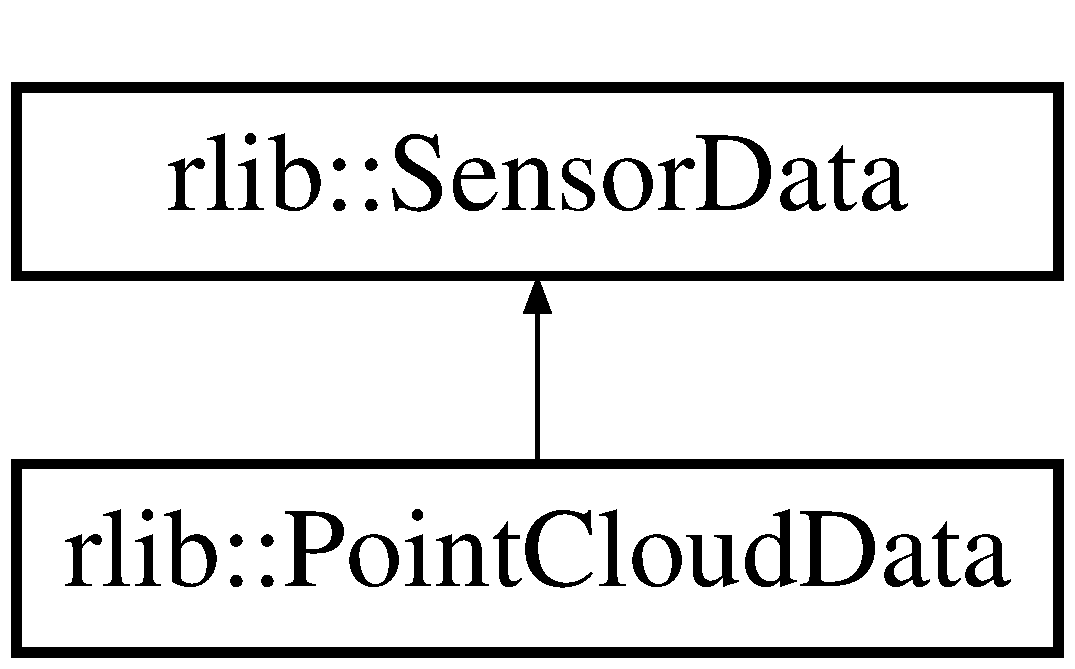
\includegraphics[height=2.000000cm]{classrlib_1_1PointCloudData}
\end{center}
\end{figure}


The documentation for this class was generated from the following file\-:\begin{DoxyCompactItemize}
\item 
include/rlib\-\_\-sensor.\-hpp\end{DoxyCompactItemize}

\hypertarget{classrlib_1_1Pose}{\section{rlib\-:\-:Pose Class Reference}
\label{classrlib_1_1Pose}\index{rlib\-::\-Pose@{rlib\-::\-Pose}}
}
\subsection*{Public Member Functions}
\begin{DoxyCompactItemize}
\item 
\hypertarget{classrlib_1_1Pose_a89018f33db4278d47440d42d515ffccb}{{\bfseries Pose} (float x, float y=0, float z=0, float roll=0, float pitch=0, float yaw=0)}\label{classrlib_1_1Pose_a89018f33db4278d47440d42d515ffccb}

\item 
\hypertarget{classrlib_1_1Pose_a5b2693a81537396e831788fb4597c908}{void {\bfseries set\-X\-Y\-Z} (float x, float y, float z)}\label{classrlib_1_1Pose_a5b2693a81537396e831788fb4597c908}

\item 
\hypertarget{classrlib_1_1Pose_a4342dd9f96dc8efe40fca92f8a6b31be}{void {\bfseries set\-R\-P\-Y} (float roll, float pitch, float yaw)}\label{classrlib_1_1Pose_a4342dd9f96dc8efe40fca92f8a6b31be}

\end{DoxyCompactItemize}
\subsection*{Public Attributes}
\begin{DoxyCompactItemize}
\item 
\hypertarget{classrlib_1_1Pose_a79943a3bc939401f14ab8feadc6f9fb0}{Eigen\-::\-Translation$<$ float, 3 $>$ {\bfseries p}}\label{classrlib_1_1Pose_a79943a3bc939401f14ab8feadc6f9fb0}

\item 
\hypertarget{classrlib_1_1Pose_ac598a727181b9ffbe5ac865239390437}{Eigen\-::\-Quaternion$<$ float $>$ {\bfseries q}}\label{classrlib_1_1Pose_ac598a727181b9ffbe5ac865239390437}

\end{DoxyCompactItemize}


The documentation for this class was generated from the following files\-:\begin{DoxyCompactItemize}
\item 
include/rlib\-\_\-state.\-hpp\item 
src/rlib\-\_\-state.\-cpp\end{DoxyCompactItemize}

\hypertarget{classrlib_1_1Robot}{\section{rlib\-:\-:Robot Class Reference}
\label{classrlib_1_1Robot}\index{rlib\-::\-Robot@{rlib\-::\-Robot}}
}
Inheritance diagram for rlib\-:\-:Robot\-:\begin{figure}[H]
\begin{center}
\leavevmode
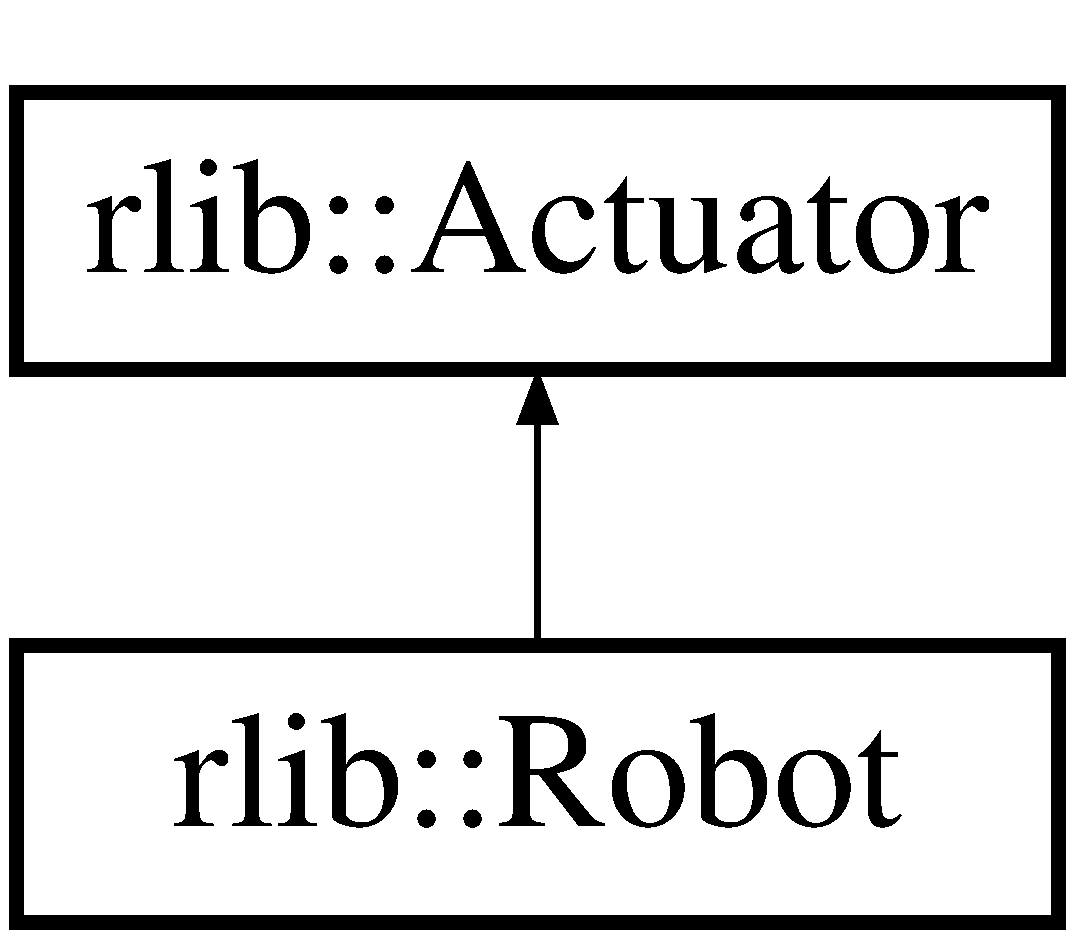
\includegraphics[height=2.000000cm]{classrlib_1_1Robot}
\end{center}
\end{figure}
\subsection*{Additional Inherited Members}


The documentation for this class was generated from the following file\-:\begin{DoxyCompactItemize}
\item 
include/rlib\-\_\-robot.\-hpp\end{DoxyCompactItemize}

\hypertarget{classrlib_1_1Sensor}{\section{rlib\-:\-:Sensor Class Reference}
\label{classrlib_1_1Sensor}\index{rlib\-::\-Sensor@{rlib\-::\-Sensor}}
}


$\ast$$\ast$$\ast$ \hyperlink{classrlib_1_1Sensor}{Sensor} Abstract Class $\ast$$\ast$$\ast$///  




{\ttfamily \#include $<$rlib\-\_\-sensor.\-hpp$>$}

Inheritance diagram for rlib\-:\-:Sensor\-:\begin{figure}[H]
\begin{center}
\leavevmode
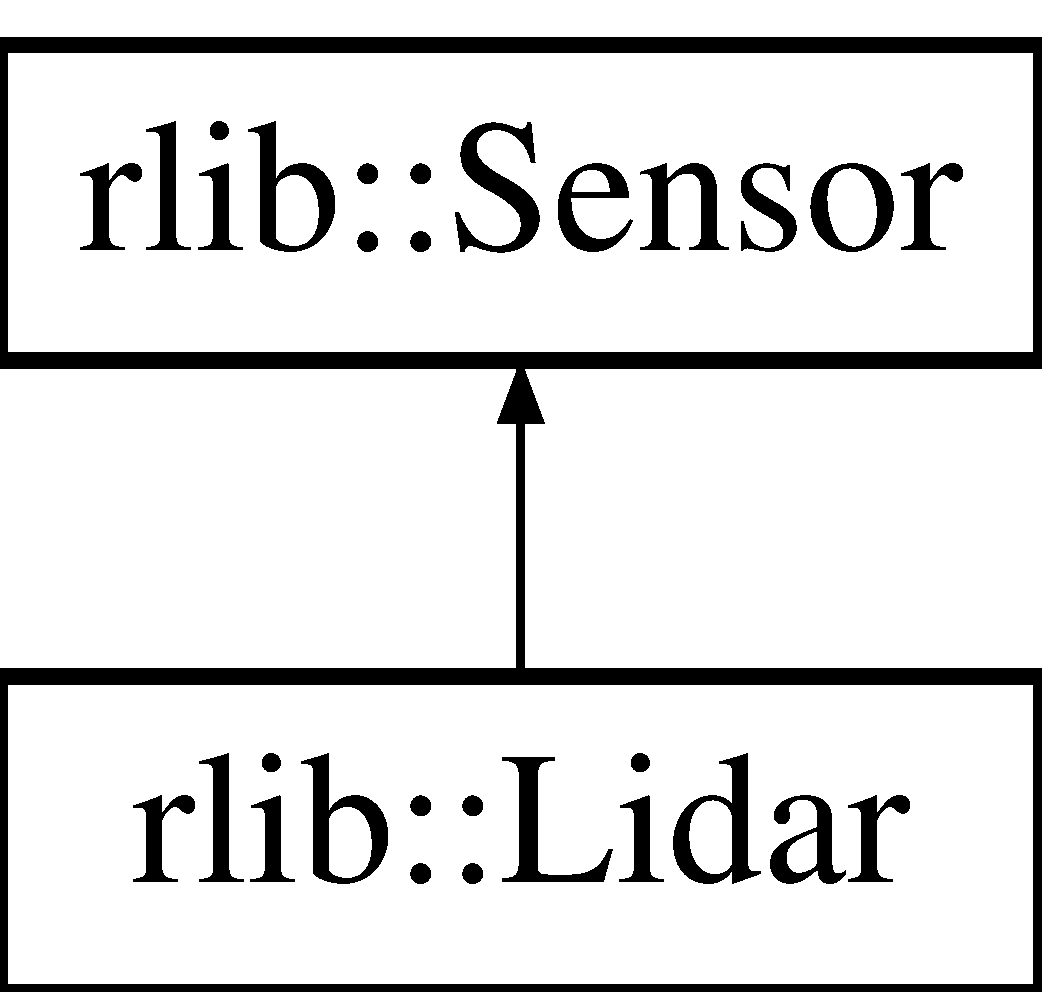
\includegraphics[height=2.000000cm]{classrlib_1_1Sensor}
\end{center}
\end{figure}
\subsection*{Public Member Functions}
\begin{DoxyCompactItemize}
\item 
\hypertarget{classrlib_1_1Sensor_a2c91acd4bed299a37f744f67e3ed1c98}{\hyperlink{classrlib_1_1Sensor_a2c91acd4bed299a37f744f67e3ed1c98}{Sensor} (const char $\ast$name)}\label{classrlib_1_1Sensor_a2c91acd4bed299a37f744f67e3ed1c98}

\begin{DoxyCompactList}\small\item\em $\ast$$\ast$$\ast$ \hyperlink{classrlib_1_1Sensor}{Sensor} Abstract Class $\ast$$\ast$$\ast$/// \end{DoxyCompactList}\item 
\hypertarget{classrlib_1_1Sensor_a398dc38404983a823704271bd78434dd}{std\-::string {\bfseries get\-Name} ()}\label{classrlib_1_1Sensor_a398dc38404983a823704271bd78434dd}

\item 
\hypertarget{classrlib_1_1Sensor_a23e53ef67e2ed8c566122576894bba21}{void {\bfseries set\-Frame} (\hyperlink{classrlib_1_1Transform}{Transform} tf)}\label{classrlib_1_1Sensor_a23e53ef67e2ed8c566122576894bba21}

\item 
\hypertarget{classrlib_1_1Sensor_a671966372280f694136d6b0880fdce33}{virtual void {\bfseries start\-Sensor} ()=0}\label{classrlib_1_1Sensor_a671966372280f694136d6b0880fdce33}

\item 
\hypertarget{classrlib_1_1Sensor_a14db3d6d3bdcac79411c1abbb6439f41}{virtual void {\bfseries stop\-Sensor} ()=0}\label{classrlib_1_1Sensor_a14db3d6d3bdcac79411c1abbb6439f41}

\item 
\hypertarget{classrlib_1_1Sensor_aff2b43bfdd9e41444000924ba72ef9c6}{virtual \hyperlink{classrlib_1_1SensorData}{Sensor\-Data} {\bfseries get\-Data} ()=0}\label{classrlib_1_1Sensor_aff2b43bfdd9e41444000924ba72ef9c6}

\end{DoxyCompactItemize}


\subsection{Detailed Description}
$\ast$$\ast$$\ast$ \hyperlink{classrlib_1_1Sensor}{Sensor} Abstract Class $\ast$$\ast$$\ast$/// 

The documentation for this class was generated from the following files\-:\begin{DoxyCompactItemize}
\item 
include/rlib\-\_\-sensor.\-hpp\item 
src/rlib\-\_\-sensor.\-cpp\end{DoxyCompactItemize}

\hypertarget{classrlib_1_1SensorData}{\section{rlib\-:\-:Sensor\-Data Class Reference}
\label{classrlib_1_1SensorData}\index{rlib\-::\-Sensor\-Data@{rlib\-::\-Sensor\-Data}}
}


$\ast$$\ast$$\ast$ \hyperlink{classrlib_1_1Sensor}{Sensor} Data Abstract Class $\ast$$\ast$$\ast$///  




{\ttfamily \#include $<$rlib\-\_\-sensor.\-hpp$>$}

Inheritance diagram for rlib\-:\-:Sensor\-Data\-:\begin{figure}[H]
\begin{center}
\leavevmode
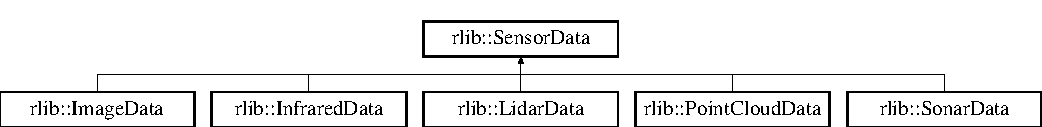
\includegraphics[height=1.709924cm]{classrlib_1_1SensorData}
\end{center}
\end{figure}


\subsection{Detailed Description}
$\ast$$\ast$$\ast$ \hyperlink{classrlib_1_1Sensor}{Sensor} Data Abstract Class $\ast$$\ast$$\ast$/// 

The documentation for this class was generated from the following file\-:\begin{DoxyCompactItemize}
\item 
include/rlib\-\_\-sensor.\-hpp\end{DoxyCompactItemize}

\hypertarget{classrlib_1_1SensorHandler}{\section{rlib\-:\-:Sensor\-Handler Class Reference}
\label{classrlib_1_1SensorHandler}\index{rlib\-::\-Sensor\-Handler@{rlib\-::\-Sensor\-Handler}}
}


Abstract class for all \hyperlink{classrlib_1_1Sensor}{Sensor} Handler objects.  




{\ttfamily \#include $<$rlib\-\_\-sensor.\-hpp$>$}

Inheritance diagram for rlib\-:\-:Sensor\-Handler\-:\begin{figure}[H]
\begin{center}
\leavevmode
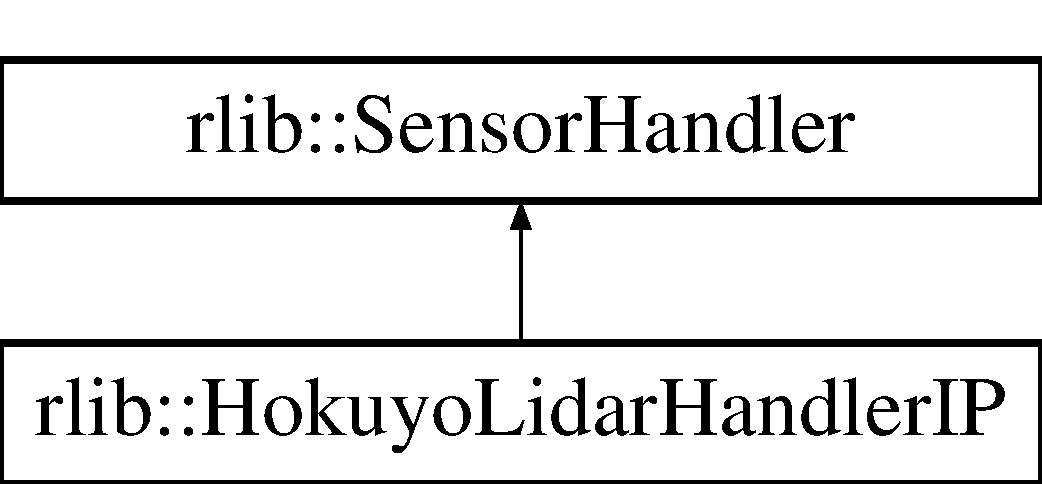
\includegraphics[height=2.000000cm]{classrlib_1_1SensorHandler}
\end{center}
\end{figure}
\subsection*{Public Member Functions}
\begin{DoxyCompactItemize}
\item 
\hyperlink{classrlib_1_1SensorHandler_ace170c82c91c36497a1a486979ebba71}{Sensor\-Handler} ()
\begin{DoxyCompactList}\small\item\em Default Handler constructor. \end{DoxyCompactList}\item 
\hypertarget{classrlib_1_1SensorHandler_a48b4756a0838c3c26b2c6d71858c588f}{virtual void \hyperlink{classrlib_1_1SensorHandler_a48b4756a0838c3c26b2c6d71858c588f}{start\-Sensor} ()=0}\label{classrlib_1_1SensorHandler_a48b4756a0838c3c26b2c6d71858c588f}

\begin{DoxyCompactList}\small\item\em Initializes and starts sensor. \end{DoxyCompactList}\item 
\hypertarget{classrlib_1_1SensorHandler_aed535cfe7182f006c9df0f02b0a48dde}{virtual void \hyperlink{classrlib_1_1SensorHandler_aed535cfe7182f006c9df0f02b0a48dde}{stop\-Sensor} ()=0}\label{classrlib_1_1SensorHandler_aed535cfe7182f006c9df0f02b0a48dde}

\begin{DoxyCompactList}\small\item\em Stops sensor. \end{DoxyCompactList}\item 
virtual \hyperlink{classrlib_1_1SensorData}{Sensor\-Data} $\ast$ \hyperlink{classrlib_1_1SensorHandler_a7f9c3e855f436aab794969b3b5cc3193}{get\-Data} ()=0
\begin{DoxyCompactList}\small\item\em Gets data from the sensor. \end{DoxyCompactList}\end{DoxyCompactItemize}


\subsection{Detailed Description}
Abstract class for all \hyperlink{classrlib_1_1Sensor}{Sensor} Handler objects. 

This is the abstract class for building all \hyperlink{classrlib_1_1Sensor}{Sensor} Handlers. These objects are meant to deal with the implementation details of actually getting sensor data. The \hyperlink{classrlib_1_1Sensor}{Sensor} Handler is kept by the \hyperlink{classrlib_1_1Sensor}{Sensor} object and uses it to get sensor data. 

\subsection{Constructor \& Destructor Documentation}
\hypertarget{classrlib_1_1SensorHandler_ace170c82c91c36497a1a486979ebba71}{\index{rlib\-::\-Sensor\-Handler@{rlib\-::\-Sensor\-Handler}!Sensor\-Handler@{Sensor\-Handler}}
\index{Sensor\-Handler@{Sensor\-Handler}!rlib::SensorHandler@{rlib\-::\-Sensor\-Handler}}
\subsubsection[{Sensor\-Handler}]{\setlength{\rightskip}{0pt plus 5cm}rlib\-::\-Sensor\-Handler\-::\-Sensor\-Handler (
\begin{DoxyParamCaption}
{}
\end{DoxyParamCaption}
)}}\label{classrlib_1_1SensorHandler_ace170c82c91c36497a1a486979ebba71}


Default Handler constructor. 

$\ast$$\ast$$\ast$ \hyperlink{classrlib_1_1Sensor}{Sensor} Handler Class $\ast$$\ast$$\ast$/// 

\subsection{Member Function Documentation}
\hypertarget{classrlib_1_1SensorHandler_a7f9c3e855f436aab794969b3b5cc3193}{\index{rlib\-::\-Sensor\-Handler@{rlib\-::\-Sensor\-Handler}!get\-Data@{get\-Data}}
\index{get\-Data@{get\-Data}!rlib::SensorHandler@{rlib\-::\-Sensor\-Handler}}
\subsubsection[{get\-Data}]{\setlength{\rightskip}{0pt plus 5cm}virtual {\bf Sensor\-Data}$\ast$ rlib\-::\-Sensor\-Handler\-::get\-Data (
\begin{DoxyParamCaption}
{}
\end{DoxyParamCaption}
)\hspace{0.3cm}{\ttfamily [pure virtual]}}}\label{classrlib_1_1SensorHandler_a7f9c3e855f436aab794969b3b5cc3193}


Gets data from the sensor. 

Requests new data from the sensor. This is a blocking function. \begin{DoxyReturn}{Returns}
The sensor data packed into the \hyperlink{classrlib_1_1SensorData}{rlib\-::\-Sensor\-Data} format. 
\end{DoxyReturn}


Implemented in \hyperlink{classrlib_1_1HokuyoLidarHandlerIP_af1b24513e31b16fb97b9a9124f29bc40}{rlib\-::\-Hokuyo\-Lidar\-Handler\-I\-P}.



The documentation for this class was generated from the following files\-:\begin{DoxyCompactItemize}
\item 
include/rlib\-\_\-sensor.\-hpp\item 
src/rlib\-\_\-sensor.\-cpp\end{DoxyCompactItemize}

\hypertarget{classrlib_1_1SonarData}{\section{rlib\-:\-:Sonar\-Data Class Reference}
\label{classrlib_1_1SonarData}\index{rlib\-::\-Sonar\-Data@{rlib\-::\-Sonar\-Data}}
}
Inheritance diagram for rlib\-:\-:Sonar\-Data\-:\begin{figure}[H]
\begin{center}
\leavevmode
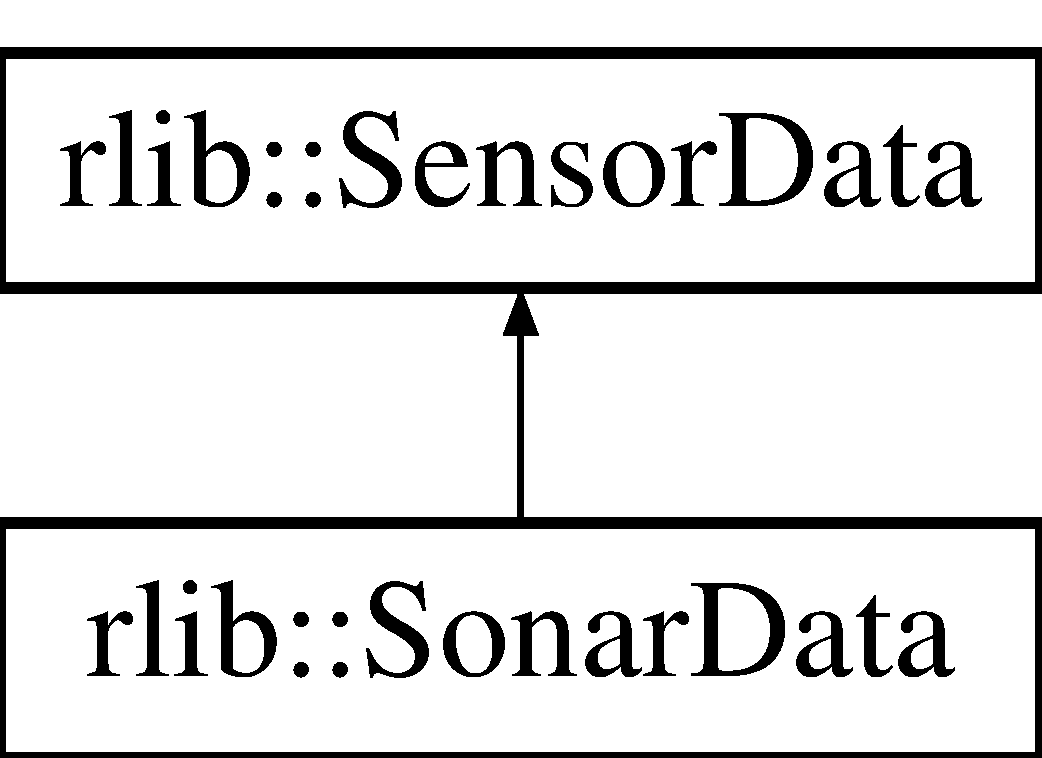
\includegraphics[height=2.000000cm]{classrlib_1_1SonarData}
\end{center}
\end{figure}


The documentation for this class was generated from the following file\-:\begin{DoxyCompactItemize}
\item 
include/rlib\-\_\-sensor.\-hpp\end{DoxyCompactItemize}

\hypertarget{classhokuyo_1_1tcp__client}{\section{hokuyo\-:\-:tcp\-\_\-client Class Reference}
\label{classhokuyo_1_1tcp__client}\index{hokuyo\-::tcp\-\_\-client@{hokuyo\-::tcp\-\_\-client}}
}


Hokuyo laser client.  




{\ttfamily \#include $<$hokuyo\-\_\-client.\-hpp$>$}

\subsection*{Public Member Functions}
\begin{DoxyCompactItemize}
\item 
\hypertarget{classhokuyo_1_1tcp__client_a8ffbb91db68f99829b3cd64e9875ce25}{const size\-\_\-t \hyperlink{classhokuyo_1_1tcp__client_a8ffbb91db68f99829b3cd64e9875ce25}{size} ()}\label{classhokuyo_1_1tcp__client_a8ffbb91db68f99829b3cd64e9875ce25}

\begin{DoxyCompactList}\small\item\em returns the number of available angle/distance pairs \end{DoxyCompactList}\item 
\hypertarget{classhokuyo_1_1tcp__client_a3b0554fedfa5db82eb7dd98321e84c54}{const fbuffer \& \hyperlink{classhokuyo_1_1tcp__client_a3b0554fedfa5db82eb7dd98321e84c54}{get\-\_\-angles} ()}\label{classhokuyo_1_1tcp__client_a3b0554fedfa5db82eb7dd98321e84c54}

\begin{DoxyCompactList}\small\item\em returns vector of angle (valid if \hyperlink{classhokuyo_1_1tcp__client_a130f57b5d6d61da417b3cbaac82c2afc}{avail()}==true) \end{DoxyCompactList}\item 
\hypertarget{classhokuyo_1_1tcp__client_accf06626b62b055ed25d2917059df73e}{const fbuffer \& \hyperlink{classhokuyo_1_1tcp__client_accf06626b62b055ed25d2917059df73e}{get\-\_\-distances} ()}\label{classhokuyo_1_1tcp__client_accf06626b62b055ed25d2917059df73e}

\begin{DoxyCompactList}\small\item\em returns vector distances (valid if \hyperlink{classhokuyo_1_1tcp__client_a130f57b5d6d61da417b3cbaac82c2afc}{avail()}==true) \end{DoxyCompactList}\item 
\hypertarget{classhokuyo_1_1tcp__client_ab35989483cd8411fe7a634ab8a15057f}{const float \& \hyperlink{classhokuyo_1_1tcp__client_ab35989483cd8411fe7a634ab8a15057f}{get\-\_\-angle} (const size\-\_\-t idx)}\label{classhokuyo_1_1tcp__client_ab35989483cd8411fe7a634ab8a15057f}

\begin{DoxyCompactList}\small\item\em returns (idx)th angle \end{DoxyCompactList}\item 
\hypertarget{classhokuyo_1_1tcp__client_ab36272194ed32fa9c96a89d80cb85fb0}{const float \& \hyperlink{classhokuyo_1_1tcp__client_ab36272194ed32fa9c96a89d80cb85fb0}{get\-\_\-distance} (const size\-\_\-t idx)}\label{classhokuyo_1_1tcp__client_ab36272194ed32fa9c96a89d80cb85fb0}

\begin{DoxyCompactList}\small\item\em returns (jdx)th distance \end{DoxyCompactList}\item 
\hypertarget{classhokuyo_1_1tcp__client_af9932c00ecbaede65b6a1cd60073e28c}{const size\-\_\-t \& \hyperlink{classhokuyo_1_1tcp__client_af9932c00ecbaede65b6a1cd60073e28c}{get\-\_\-frame\-\_\-count} ()}\label{classhokuyo_1_1tcp__client_af9932c00ecbaede65b6a1cd60073e28c}

\begin{DoxyCompactList}\small\item\em returns the number of recieved frames \end{DoxyCompactList}\item 
\hypertarget{classhokuyo_1_1tcp__client_aa6e3e44f43147facd7414f9f0e03fc61}{const size\-\_\-t \& \hyperlink{classhokuyo_1_1tcp__client_aa6e3e44f43147facd7414f9f0e03fc61}{get\-\_\-missed\-\_\-count} ()}\label{classhokuyo_1_1tcp__client_aa6e3e44f43147facd7414f9f0e03fc61}

\begin{DoxyCompactList}\small\item\em returns the number of incomplete/faulty frames \end{DoxyCompactList}\item 
\hypertarget{classhokuyo_1_1tcp__client_a6049b6fc4e800b0b580d5ce32f95e5b3}{float {\bfseries get\-\_\-max\-\_\-range} ()}\label{classhokuyo_1_1tcp__client_a6049b6fc4e800b0b580d5ce32f95e5b3}

\item 
\hypertarget{classhokuyo_1_1tcp__client_acb30c8e726535bc5467675fbeedfa4cd}{float {\bfseries get\-\_\-min\-\_\-range} ()}\label{classhokuyo_1_1tcp__client_acb30c8e726535bc5467675fbeedfa4cd}

\item 
void \hyperlink{classhokuyo_1_1tcp__client_a43b62c13de109820ab4e804efd76a95c}{start} ()
\begin{DoxyCompactList}\small\item\em starts server communication process \end{DoxyCompactList}\item 
void \hyperlink{classhokuyo_1_1tcp__client_ab54b7c58e9ad125e42624744e26d22d4}{stop} ()
\begin{DoxyCompactList}\small\item\em ends server communication process \end{DoxyCompactList}\item 
\hypertarget{classhokuyo_1_1tcp__client_a43cf16989bd80fece9849064ecd284b6}{void \hyperlink{classhokuyo_1_1tcp__client_a43cf16989bd80fece9849064ecd284b6}{request} ()}\label{classhokuyo_1_1tcp__client_a43cf16989bd80fece9849064ecd284b6}

\begin{DoxyCompactList}\small\item\em request a new aquisition \end{DoxyCompactList}\item 
\hypertarget{classhokuyo_1_1tcp__client_a130f57b5d6d61da417b3cbaac82c2afc}{bool \hyperlink{classhokuyo_1_1tcp__client_a130f57b5d6d61da417b3cbaac82c2afc}{avail} ()}\label{classhokuyo_1_1tcp__client_a130f57b5d6d61da417b3cbaac82c2afc}

\begin{DoxyCompactList}\small\item\em returns true if 'data-\/flag' is set \end{DoxyCompactList}\item 
\hypertarget{classhokuyo_1_1tcp__client_adcb05f1bd91648a1971d55fb0f3795d7}{bool \hyperlink{classhokuyo_1_1tcp__client_adcb05f1bd91648a1971d55fb0f3795d7}{valid} ()}\label{classhokuyo_1_1tcp__client_adcb05f1bd91648a1971d55fb0f3795d7}

\begin{DoxyCompactList}\small\item\em returns true if \hyperlink{classhokuyo_1_1tcp__client_a130f57b5d6d61da417b3cbaac82c2afc}{avail()} and buffer has correct number of elements \end{DoxyCompactList}\item 
\hyperlink{classhokuyo_1_1tcp__client_a1890aa338d5513f3a7f8a8d05d2c7f18}{tcp\-\_\-client} (const char $\ast$address, const char $\ast$port, asio\-::ip\-::tcp\-::socket \&socket)
\begin{DoxyCompactList}\small\item\em Default constructor; sets up connection to client. \end{DoxyCompactList}\item 
\hypertarget{classhokuyo_1_1tcp__client_ad3a0b2ba1df3334d3ea0710597c7ac71}{virtual \hyperlink{classhokuyo_1_1tcp__client_ad3a0b2ba1df3334d3ea0710597c7ac71}{$\sim$tcp\-\_\-client} ()}\label{classhokuyo_1_1tcp__client_ad3a0b2ba1df3334d3ea0710597c7ac71}

\begin{DoxyCompactList}\small\item\em Closes socket comms upon deletion. \end{DoxyCompactList}\end{DoxyCompactItemize}
\subsection*{Friends}
\begin{DoxyCompactItemize}
\item 
\hypertarget{classhokuyo_1_1tcp__client_a265e70855ac77efd577b4a3a0ac8830f}{std\-::ostream \& {\bfseries operator$<$$<$} (std\-::ostream \&os, \hyperlink{classhokuyo_1_1tcp__client}{tcp\-\_\-client} \&cli)}\label{classhokuyo_1_1tcp__client_a265e70855ac77efd577b4a3a0ac8830f}

\item 
void \hyperlink{classhokuyo_1_1tcp__client_af9807b92251be2aa065324c2edbd9ac3}{tcp\-\_\-client\-\_\-read\-\_\-service} (\hyperlink{classhokuyo_1_1tcp__client}{tcp\-\_\-client} $\ast$cli)
\end{DoxyCompactItemize}


\subsection{Detailed Description}
Hokuyo laser client. 

\subsection{Constructor \& Destructor Documentation}
\hypertarget{classhokuyo_1_1tcp__client_a1890aa338d5513f3a7f8a8d05d2c7f18}{\index{hokuyo\-::tcp\-\_\-client@{hokuyo\-::tcp\-\_\-client}!tcp\-\_\-client@{tcp\-\_\-client}}
\index{tcp\-\_\-client@{tcp\-\_\-client}!hokuyo::tcp_client@{hokuyo\-::tcp\-\_\-client}}
\subsubsection[{tcp\-\_\-client}]{\setlength{\rightskip}{0pt plus 5cm}hokuyo\-::tcp\-\_\-client\-::tcp\-\_\-client (
\begin{DoxyParamCaption}
\item[{const char $\ast$}]{address, }
\item[{const char $\ast$}]{port, }
\item[{asio\-::ip\-::tcp\-::socket \&}]{socket}
\end{DoxyParamCaption}
)\hspace{0.3cm}{\ttfamily [explicit]}}}\label{classhokuyo_1_1tcp__client_a1890aa338d5513f3a7f8a8d05d2c7f18}


Default constructor; sets up connection to client. 


\begin{DoxyParams}[1]{Parameters}
\mbox{\tt in}  & {\em address} & server's ip address \\
\hline
\mbox{\tt in}  & {\em port} & commincation port \\
\hline
 & {\em \mbox{[}in} & socket socket object thru which comms are performed \\
\hline
\end{DoxyParams}


\subsection{Member Function Documentation}
\hypertarget{classhokuyo_1_1tcp__client_a43b62c13de109820ab4e804efd76a95c}{\index{hokuyo\-::tcp\-\_\-client@{hokuyo\-::tcp\-\_\-client}!start@{start}}
\index{start@{start}!hokuyo::tcp_client@{hokuyo\-::tcp\-\_\-client}}
\subsubsection[{start}]{\setlength{\rightskip}{0pt plus 5cm}void hokuyo\-::tcp\-\_\-client\-::start (
\begin{DoxyParamCaption}
{}
\end{DoxyParamCaption}
)}}\label{classhokuyo_1_1tcp__client_a43b62c13de109820ab4e804efd76a95c}


starts server communication process 

If a job is not active... \hypertarget{classhokuyo_1_1tcp__client_ab54b7c58e9ad125e42624744e26d22d4}{\index{hokuyo\-::tcp\-\_\-client@{hokuyo\-::tcp\-\_\-client}!stop@{stop}}
\index{stop@{stop}!hokuyo::tcp_client@{hokuyo\-::tcp\-\_\-client}}
\subsubsection[{stop}]{\setlength{\rightskip}{0pt plus 5cm}void hokuyo\-::tcp\-\_\-client\-::stop (
\begin{DoxyParamCaption}
{}
\end{DoxyParamCaption}
)}}\label{classhokuyo_1_1tcp__client_ab54b7c58e9ad125e42624744e26d22d4}


ends server communication process 

If a job has been started..

Reset frame counters

Cleanup the service on server side 

\subsection{Friends And Related Function Documentation}
\hypertarget{classhokuyo_1_1tcp__client_af9807b92251be2aa065324c2edbd9ac3}{\index{hokuyo\-::tcp\-\_\-client@{hokuyo\-::tcp\-\_\-client}!tcp\-\_\-client\-\_\-read\-\_\-service@{tcp\-\_\-client\-\_\-read\-\_\-service}}
\index{tcp\-\_\-client\-\_\-read\-\_\-service@{tcp\-\_\-client\-\_\-read\-\_\-service}!hokuyo::tcp_client@{hokuyo\-::tcp\-\_\-client}}
\subsubsection[{tcp\-\_\-client\-\_\-read\-\_\-service}]{\setlength{\rightskip}{0pt plus 5cm}void tcp\-\_\-client\-\_\-read\-\_\-service (
\begin{DoxyParamCaption}
\item[{{\bf tcp\-\_\-client} $\ast$}]{cli}
\end{DoxyParamCaption}
)\hspace{0.3cm}{\ttfamily [friend]}}}\label{classhokuyo_1_1tcp__client_af9807b92251be2aa065324c2edbd9ac3}
Initiate serial on server side

Run service as long as thread lives

Sleep

Check if read requested

Initiate transimission by request

Data is not ready

Clear old data

Begin reading frame

Get size field

Get data bytes + convert to floats

Convert byte stream to floats

Push data to angle/distance vectors

Check the state of transmission
\begin{DoxyItemize}
\item There should be no bytes avail if a request was fully processed
\end{DoxyItemize}

Data is ready 

The documentation for this class was generated from the following files\-:\begin{DoxyCompactItemize}
\item 
include/hokuyo\-\_\-client.\-hpp\item 
src/hokuyo\-\_\-client.\-cpp\end{DoxyCompactItemize}

\hypertarget{classrlib_1_1Transform}{\section{rlib\-:\-:Transform Class Reference}
\label{classrlib_1_1Transform}\index{rlib\-::\-Transform@{rlib\-::\-Transform}}
}
\subsection*{Public Attributes}
\begin{DoxyCompactItemize}
\item 
\hypertarget{classrlib_1_1Transform_a38135d56804225fa5e1bac5a5c6b3d9d}{Eigen\-::\-Transform$<$ float, \\*
3, Eigen\-::\-Affine $>$ {\bfseries T}}\label{classrlib_1_1Transform_a38135d56804225fa5e1bac5a5c6b3d9d}

\end{DoxyCompactItemize}


The documentation for this class was generated from the following file\-:\begin{DoxyCompactItemize}
\item 
include/rlib\-\_\-state.\-hpp\end{DoxyCompactItemize}

\hypertarget{classrlib_1_1Vel}{\section{rlib\-:\-:Vel Class Reference}
\label{classrlib_1_1Vel}\index{rlib\-::\-Vel@{rlib\-::\-Vel}}
}


Class for defining velocities.  




{\ttfamily \#include $<$rlib\-\_\-state.\-hpp$>$}

\subsection*{Public Attributes}
\begin{DoxyCompactItemize}
\item 
float \hyperlink{classrlib_1_1Vel_aba9035c6e774edd37f2421ec376bb8f3}{vx}
\item 
float \hyperlink{classrlib_1_1Vel_acb4d80d6a58e1813359f9931d2fc6c9e}{vy}
\item 
float \hyperlink{classrlib_1_1Vel_aab3819a2079bb4654939da51cf896af3}{vz}
\item 
float \hyperlink{classrlib_1_1Vel_adc2bc037dd0c69f0aaa972a41b8af55c}{wx}
\item 
float \hyperlink{classrlib_1_1Vel_a40c6bb36dcb99cd88214e92c8169e7b1}{wy}
\item 
float \hyperlink{classrlib_1_1Vel_a7f1cf4b7d0dba121ec54d0011eb1e4d5}{wz}
\end{DoxyCompactItemize}


\subsection{Detailed Description}
Class for defining velocities. 

\subsection{Member Data Documentation}
\hypertarget{classrlib_1_1Vel_aba9035c6e774edd37f2421ec376bb8f3}{\index{rlib\-::\-Vel@{rlib\-::\-Vel}!vx@{vx}}
\index{vx@{vx}!rlib::Vel@{rlib\-::\-Vel}}
\subsubsection[{vx}]{\setlength{\rightskip}{0pt plus 5cm}float rlib\-::\-Vel\-::vx}}\label{classrlib_1_1Vel_aba9035c6e774edd37f2421ec376bb8f3}
Linear velocities in the x-\/axis in m/s. \hypertarget{classrlib_1_1Vel_acb4d80d6a58e1813359f9931d2fc6c9e}{\index{rlib\-::\-Vel@{rlib\-::\-Vel}!vy@{vy}}
\index{vy@{vy}!rlib::Vel@{rlib\-::\-Vel}}
\subsubsection[{vy}]{\setlength{\rightskip}{0pt plus 5cm}float rlib\-::\-Vel\-::vy}}\label{classrlib_1_1Vel_acb4d80d6a58e1813359f9931d2fc6c9e}
Linear velocities in the y-\/axis in m/s. \hypertarget{classrlib_1_1Vel_aab3819a2079bb4654939da51cf896af3}{\index{rlib\-::\-Vel@{rlib\-::\-Vel}!vz@{vz}}
\index{vz@{vz}!rlib::Vel@{rlib\-::\-Vel}}
\subsubsection[{vz}]{\setlength{\rightskip}{0pt plus 5cm}float rlib\-::\-Vel\-::vz}}\label{classrlib_1_1Vel_aab3819a2079bb4654939da51cf896af3}
Linear velocities in the z-\/axis in m/s. \hypertarget{classrlib_1_1Vel_adc2bc037dd0c69f0aaa972a41b8af55c}{\index{rlib\-::\-Vel@{rlib\-::\-Vel}!wx@{wx}}
\index{wx@{wx}!rlib::Vel@{rlib\-::\-Vel}}
\subsubsection[{wx}]{\setlength{\rightskip}{0pt plus 5cm}float rlib\-::\-Vel\-::wx}}\label{classrlib_1_1Vel_adc2bc037dd0c69f0aaa972a41b8af55c}
Angular velocities in the x-\/axis in rad/s. \hypertarget{classrlib_1_1Vel_a40c6bb36dcb99cd88214e92c8169e7b1}{\index{rlib\-::\-Vel@{rlib\-::\-Vel}!wy@{wy}}
\index{wy@{wy}!rlib::Vel@{rlib\-::\-Vel}}
\subsubsection[{wy}]{\setlength{\rightskip}{0pt plus 5cm}float rlib\-::\-Vel\-::wy}}\label{classrlib_1_1Vel_a40c6bb36dcb99cd88214e92c8169e7b1}
Angular velocities in the y-\/axis in rad/s. \hypertarget{classrlib_1_1Vel_a7f1cf4b7d0dba121ec54d0011eb1e4d5}{\index{rlib\-::\-Vel@{rlib\-::\-Vel}!wz@{wz}}
\index{wz@{wz}!rlib::Vel@{rlib\-::\-Vel}}
\subsubsection[{wz}]{\setlength{\rightskip}{0pt plus 5cm}float rlib\-::\-Vel\-::wz}}\label{classrlib_1_1Vel_a7f1cf4b7d0dba121ec54d0011eb1e4d5}
Angular velocities in the z-\/axis in rad/s. 

The documentation for this class was generated from the following file\-:\begin{DoxyCompactItemize}
\item 
include/rlib\-\_\-state.\-hpp\end{DoxyCompactItemize}

%--- End generated contents ---

% Index
\newpage
\phantomsection
\addcontentsline{toc}{chapter}{Index}
\printindex

\end{document}
